%%%%%%%%%%%%%%%%%%%%%%%%%%%%%%%%%%%%%%%%%%%%%%%%%%%
%% Guideline for Ontology Development in the IoP 
%% Lina Teresa Molinas Comet September 2022 <linamolinascomet@protonmail.com>
%%%%%%%%%%%%%%%%%%%%%%%%%%%%%%%%%%%%%%%%%%%%%%%%%%%
%% Document Class
\documentclass{guideline/sty/rapport}

\title{Guidelines for the creation of semantic models in the IoP}

\author{
	Lina Teresa Molinas Comet
}

\advisor[Reviewers]{
	Patrick Sapel, M.Sc. \\
	Iraklis Dimitriadis, M.Sc.
}


%%%%%%%%%%%%%%%%%%%%%%%%%%%%%%%%%%%%%%%%%%%%%%%%%%%
%% Bibliography
%%%%%%%%%%%%%%%%%%%%%%%%%%%%%%%%%%%%%%%%%%%%%%%%%%%
\addbibresource{bibliography.bib}


%%%%%%%%%%%%%%%%%%%%%%%%%%%%%%%%%%%%%%%%%%%%%%%%%%%
%% Begin Document
%%%%%%%%%%%%%%%%%%%%%%%%%%%%%%%%%%%%%%%%%%%%%%%%%%%
\begin{document} 

% Title of the document
\maketitle

\section*{Version Control Table}
\begin{table}[H]
	\centering
	\rowcolors{1}{unitednationsblue!20}{}
	\begin{tabular}{L{.09\textwidth} L{.25\textwidth} L{.10\textwidth}  L{.40\textwidth}}
		\hline
		\rowcolor{oceanboatblue!20} 
		\textbf{Version} & \textbf{Author} & \textbf{Date} & \textbf{Changes}  \\
		\hline
		V 0.1 & Lina Molinas Comet & 28.07.2022 & First draft \\
		V 0.2 & Lina Molinas Comet & 01.08.2022 & Add more catalogues \\
		V 0.3 & Lina Molinas Comet & 03.08.2022 & Modify methodology figures, add additional tools \\
		V 0.3 & Lina Molinas Comet & 01.09.2022 & Add hints in the workflow and additional examples \\
		\hline
	\end{tabular}
\end{table}

In case of questions regarding this guideline, please contact one of the following contact persons: \singlespacing
\begin{itemize}
	\item Lina Teresa Molinas Comet
	\begin{itemize}
			\item \href{mailto:lina.molinas.comet@rwth-aachen.de}{lina.molinas.comet@rwth-aachen.de} or  
			\item \href{mailto:linamolinascomet@protonmail.com}{linamolinascomet@protonmail.com} 
		\end{itemize}
	\item Patrick Sapel \href{mailto:Patrick.Sapel@ikv.rwth-aachen.de}{Patrick.Sapel@ikv.rwth-aachen.de}
    \item Iraklis Dimitriadis \href{mailto:iraklis.dimitriadis@fit.fraunhofer.de}{iraklis.dimitriadis@fit.fraunhofer.de}
\end{itemize}


%Less strict justification: prevents some words from protruding into the margin
\sloppy  


%%%%%%%%%%%%%%%%%%%%%%%%%%%%%%%%%%%%%%%%%%%%%%%%%%%
%% List of Abbreviations
%%%%%%%%%%%%%%%%%%%%%%%%%%%%%%%%%%%%%%%%%%%%%%%%%%%
\section*{List of Abbreviations}

\begin{acronym}[OntoDevMethodologies]\itemsep=5.5pt
 \acro{CQs}{Competency Questions}
 \acro{CWA}{Closed-World Assumption}
 \acro{DE}{Domain Expert}
 \acro{DEs}{Domain Experts}
 \acro{ER}{Entity-relationship}
 \acro{FAIR}{Findable, Accessible, Interoperable and Reusable}
 \acro{KE}{Knowledge Engineer}
 \acro{KEs}{Knowledge Engineers}
 \acro{KG}{Knowledge Graph}
 \acro{KGs}{Knowledge Graphs}
 \acro{I4.0}{Industry 4.0}
 \acro{IKV}{Institute for Plastic Processing in Industry and Craft}
 \acro{IoP}{Internet of Production}
 \acro{IoT}{Internet of Things}
 \acro{ODP}{Ontology Design Pattern}
 \acro{ODPs}{Ontology Design Patterns}
 \acro{OntoDevMethodologies}{Ontology Development Methodologies}
 \acro{OntoDevProcess}{Ontology Development Process}
 \acro{OntoDevTools}{Ontology Development Tools}
 \acro{OOP}{Object Oriented Programming}
 \acro{OOPS!}{Ontology  Pitfall  Scanner!}
 \acro{ORSD}{Ontology Requirements Specification}
 \acro{OWA}{Open-World Assumption}
 \acro{OWL}{Web Ontology Language}
 \acro{RAMI 4.0}{Reference Architecture Model for Industry 4.0}
 \acro{RDF}{Resource Description Framework}
 \acro{RDFS}{Resource Description Framework Schema}
 \acro{SHACL}{Shapes Constraint Language}
 \acro{ShEx}{Shape Expressions}
 \acro{SPARQL}{SPARQL Protocol and RDF Query Language} 
 \acro{SW}{Semantic Web}
 \acro{UNA}{Unique Name Assumption}
 \acro{URI}{Uniform Resource Identifier}
 \acro{VOWL}{Visual Notation for OWL Ontologies}
 \acro{W3C}{The World Wide Web Consortium}
 \end{acronym} 

\clearpage



%%%%%%%%%%%%%%%%%%%%%%%%%%%%%%%%%%%%%%%%%%%%%%%%%%%
%% Introduction
%%%%%%%%%%%%%%%%%%%%%%%%%%%%%%%%%%%%%%%%%%%%%%%%%%%
\section{Introduction}
\label{sec:Introduction}
\ac{I4.0} aims to enable autonomous coordination of processes and machines through interconnectivity and automation of processes \cite{Industrie40}, migrating from mass production to mass customization \cite{Psarommatis22}. In this context, the \ac{IoP} is considered to be the core of the visible rising \ac{I4.0}. \cite{InternetProduction}.\singlespacing

To achieve the goals of the \ac{I4.0}, more specifically, to enable autonomous production, it is necessary to have a semantic model, which is a formal description of the knowledge related to, in this case, the production system, work-pieces, assets, the process involved, and the environment. Indeed, to obtain an optimal and valid knowledge modelling, both groups of actors, \ac{DEs} and \ac{KEs}, must work in cooperation complementing each other's work. In particular, this is necessary as \ac{DEs} know the intricacies of the domain in the production system. However, they often lack knowledge about creating formal and syntactically correct semantic models. On the contrary, \ac{KEs} understand how to formalize knowledge representation but do not have a deep understanding of the domain they want to model.\singlespacing

In Fig. \textbf{\ref{fig:semanticsIoP}}, we show a small example of how a semantic model represents the real world, in this case, part of the manufacturing process by modelling the objects, their attributes and the necessary constraints.

\subsection{Motivation and Scope}

The first requirement for the creation of semantic models helping to achieve the goals of the \ac{IoP} is to have a guideline integrating enough information and directives on how to develop ontologies, which can be helpful for the actors involved in the process and in this way achieve coordination among them. \singlespacing

Even though there exist several methodologies for ontology development, there is no single guidebook or template that facilitates the modelling process and saves time for both groups of actors. Moreover, the approach of introducing existing methodologies is neither simple nor user-friendly.\singlespacing

The scope of this document is to provide an intuitive guideline in the form of a digital guide to help \ac{DEs} to create semantic models, more specifically ontologies, mostly on their own but still collaborating with \ac{KEs}. Also, we present an overview of existing domain-specific ontologies in the production and manufacturing domain and a catalogue of existing ontologies. Reusing existing ones instead of creating a new one from scratch will allow interoperability of the new ontology with existing ones. Our proposed guideline allows both \ac{DEs} and \ac{KEs} to work in a coordinated way to create and maintain ontologies efficiently.\singlespacing

To develop this guideline, we studied and unified best practices and existing methodologies used for ontology development. In this way, we support stakeholders who design ontologies to model knowledge on the Internet of Production (\ac{IoP}).

\begin{figure}[H]
        \centering
          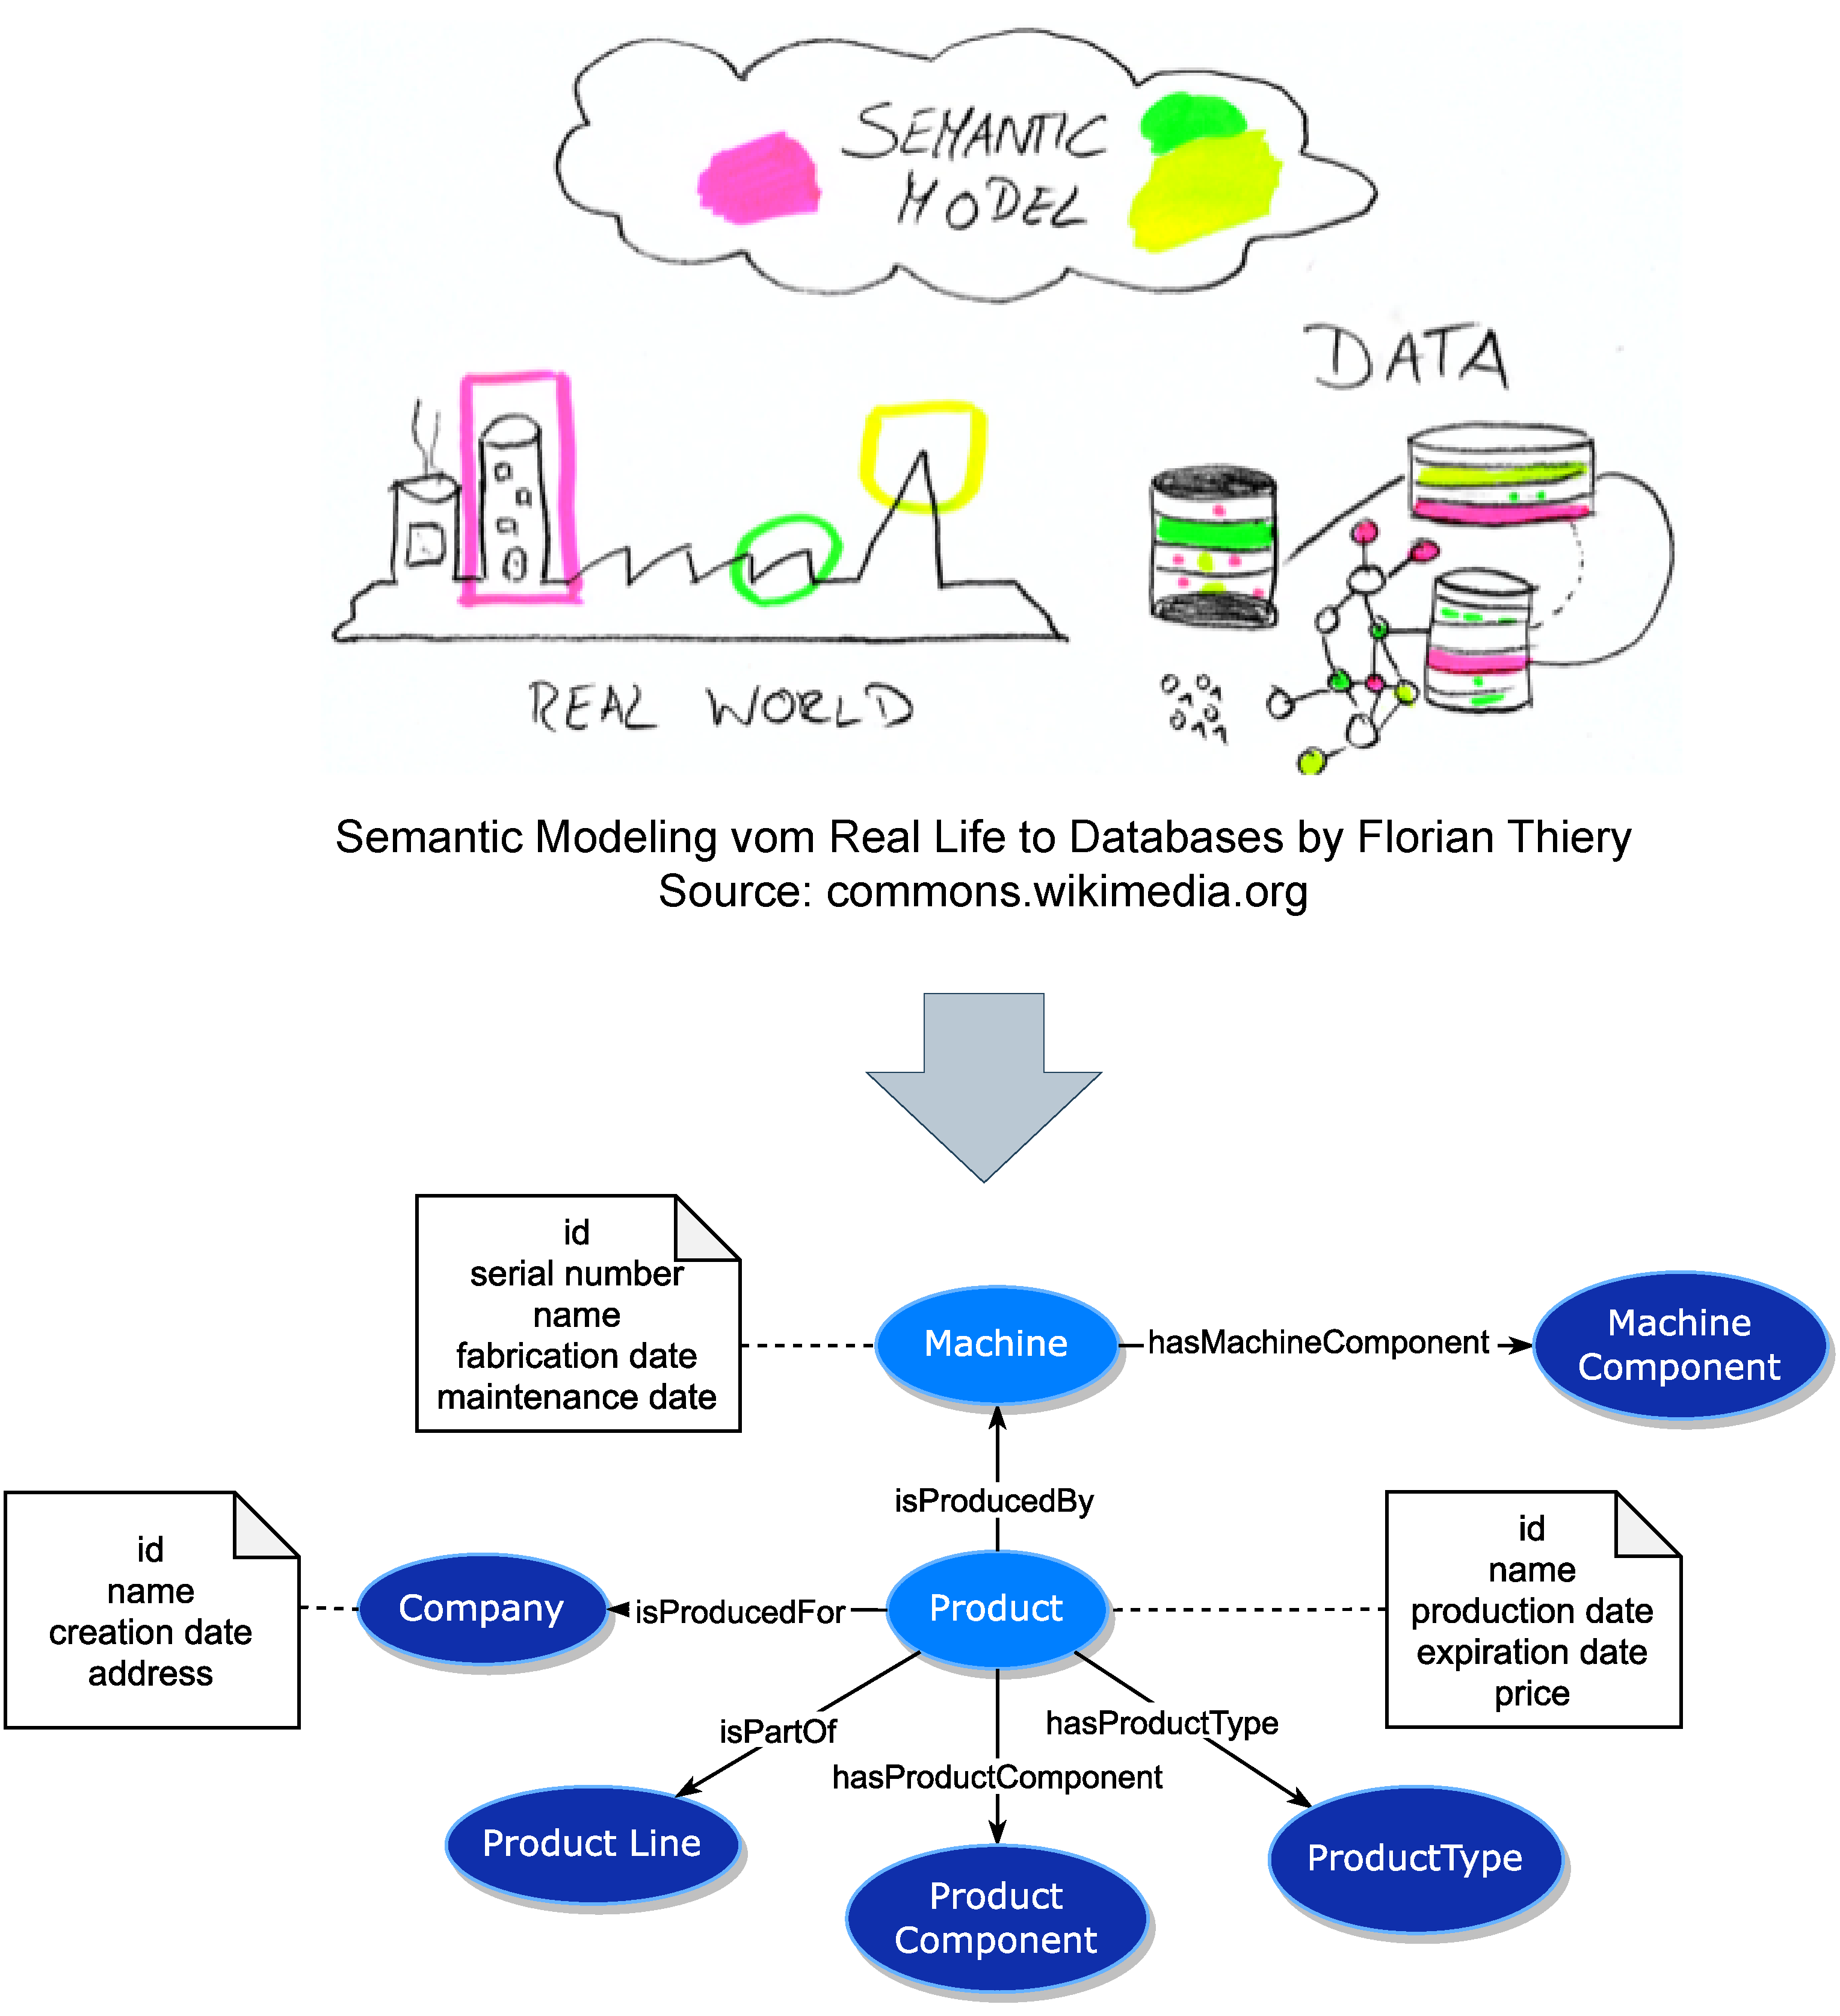
\includegraphics[width=0.9\textwidth]{images/semanticmodelabstraction.pdf}
          \caption{Semantics are needed to achieve the IoP}\label{fig:semanticsIoP}
    \end{figure}

\subsection{Audience and Use of this Guideline}
The target audience of this document extends to those involved in the ontology development process, in particular: \singlespacing

\begin{itemize}
    \item Domain Experts (DEs) in the manufacturing and production domains with little to no experience in Ontology Engineering. It will help them to create and maintain an ontology.
    \item Knowledge Experts (KEs) to support \ac{DEs} in the ontology development process when needed.
\end{itemize} \singlespacing

We should remark that while this guideline aims to be a simple and basic resource, it is beneficial to gain some knowledge about basic concepts of ontologies. Therefore, we will explain those fundamental notions in Chapter \ref{sec:fundamentals}.

\subsection{Organization of this Guideline}

Chapter \textbf{\ref{sec:Introduction}}  introduces the current problems with semantic modelling in the IoP, the target audience and the goal of this document. Chapter \textbf{\ref{sec:fundamentals}} presents the basic concepts and examples related to this guideline. We recommend that readers unfamiliar with the concepts of ontologies and semantic models first read the fundamental terminologies and explanations presented in this section because the rest of the document builds on top of it. \singlespacing

Chapter \textbf{\ref{sec:methodologies}} presents the recommended methodology to create and maintain ontologies, a workflow to indicate the different stages of the process, and some additional resources to clarify concepts and how to proceed with the ontology creation. Then, in Chapter \textbf{\ref{sec:bestpractices}}, we enumerate some of the most common best practices to consider when building ontologies to assure interoperability and reusability of the ontology. In Chapter \textbf{\ref{sec:tools}} we match the stages of the ontology development process with the corresponding tools. After that, in Chapter \textbf{\ref{sec:templates}} we provide document templates that can be used to start the process and whose content later will translate into the ontology. \singlespacing

Finally, in Chapter \textbf{\ref{sec:architecturalsuggestions}} we suggest an architectural design on how the ontology would look by providing information about existing ontologies and a catalogue to localize some of these ontologies. \singlespacing

In this chapter, we introduce the topic, motivation and scope of this guideline. Also, we detailed the structure of this document. Additionally, for a better understanding, we present a summary of how to use this guideline in Fig. \textbf{\ref{fig:howtousethisguideline}}. 

One starts by identifying the use case we want to focus on and the need for using ontologies, then continues by learning the fundamental concepts about ontologies. After that, one focuses on the suggested methodology, best practices and tools to use and uses the proposed templates. Finally, using the information from this guideline, one builds a new ontology.

    \begin{figure}[H]
        \centering
          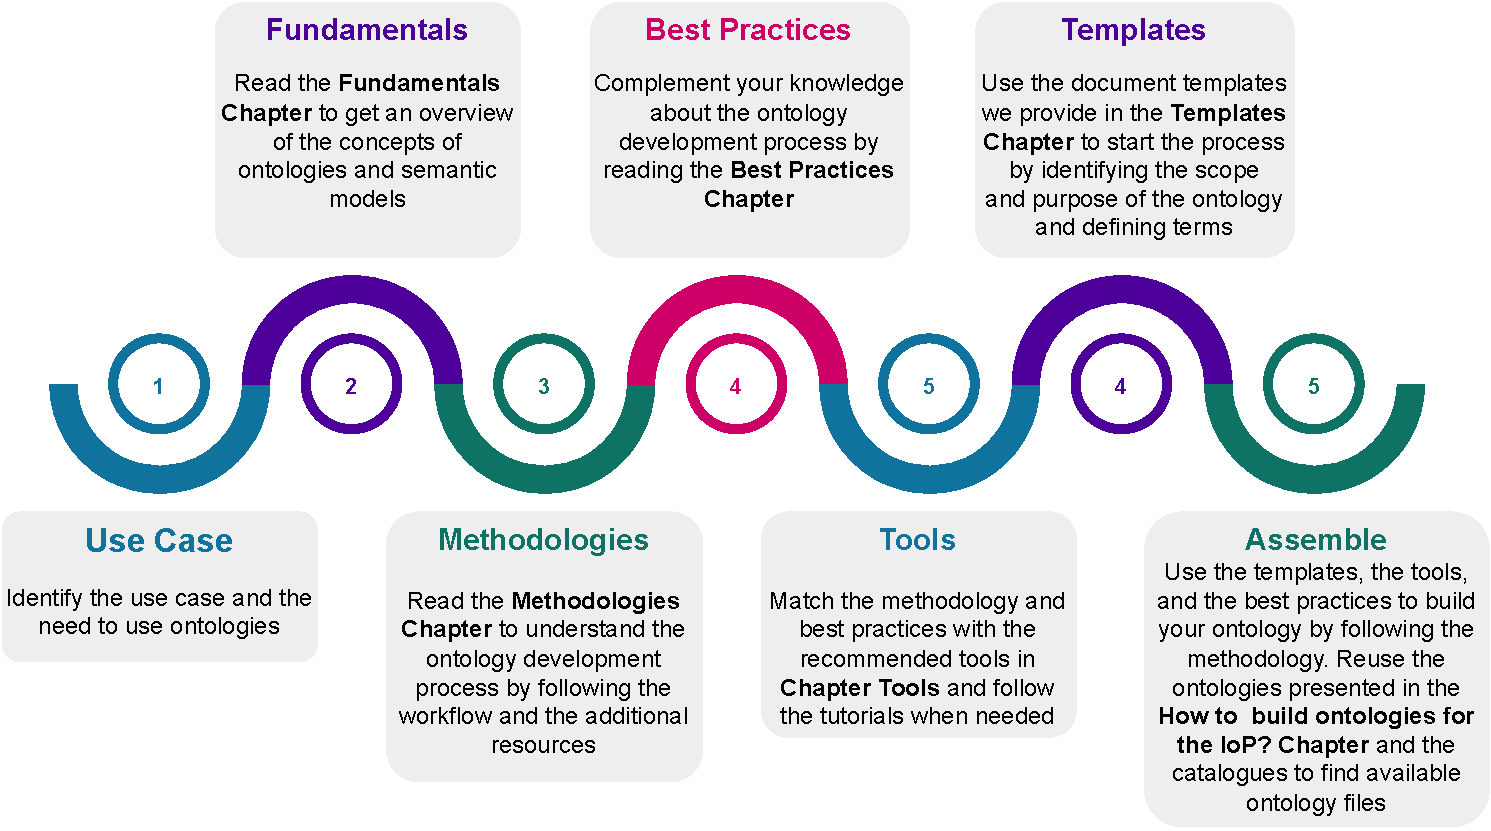
\includegraphics[width=\linewidth]{images/howtouseguideline.pdf}
          \caption{Our recommendation on how to use this guideline}
    \label{fig:howtousethisguideline}
    \end{figure}


\subsection{Notation Conventions}

We use the following formatting to express different parts of this document.

\begin{itemize}
    \item We use figures, such as Fig. \textbf{\ref{fig:semanticsIoP}} to show examples graphically, and to introduce some concepts or structures.
    \item We use \begin{beware}[Remark]
    to express important considerations.
    \end{beware}
    \item We use \begin{beware}[Note]
    to express further comments and considerations.
    \end{beware}
    \item We use tables, such as Table \textbf{\ref{tab:catalogs}} to present an overview of resources.
    \item We highlight concepts by using conceptual examples such as:
    \begin{figure}[H]
        \centering
          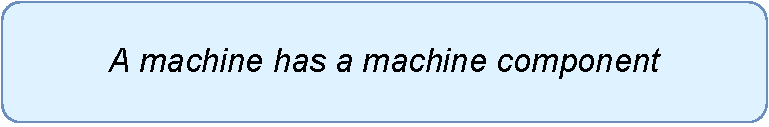
\includegraphics[width=0.5\textwidth]{images/implications0.pdf}
    \end{figure}
    \item We highlight a word or phrase to give emphasis, for example, \colorbox{bananamania}{\texttt{a highlighted phrase}}.
    \item We use references, such as Chapter \textbf{\ref{sec:fundamentals}} to refer and link to a specific resource, such as sections or figures in this document.
\end{itemize}
    
\section{Fundamentals} \label{sec:fundamentals}

%%%%%%%%%%%%%%%%%%%%%%%%%%%%%%%%%%%%%%%%%%%%%%%%%%%
%% Semantic Models
%%%%%%%%%%%%%%%%%%%%%%%%%%%%%%%%%%%%%%%%%%%%%%%%%%%

\subsection{Why are Semantic Models and Ontologies Important?}
We motivated the creation of this guideline by indicating that semantic models are needed to achieve the goals of the \ac{I4.0} and \ac{IoP}, such as autonomous production. Therefore, in this section, we first indicate why they are relevant in production and manufacturing. Later we explain their concepts and give concrete examples to support a better understanding of the concepts.  \singlespacing

Nowadays, as a large amount of data in diverse formats is available from different and distributed sources, semantic models and ontologies are necessary for achieving data integration, and more specifically, semantic interoperability\footnote{Semantic interoperability refers to the ability of systems to share a common understanding of concepts} \cite{Wache01}. It is feasible to attain this goal because ontologies help to specify a shared definition of concepts, and therefore a higher level of abstraction is achieved. Furthermore, it is possible to apply reasoning techniques to semantic models and extract knowledge, make predictions and support decision-making by implying knowledge \cite{Noy01, Psarommatis22}, as we will show in the examples in the upcoming sections. 

\subsection{How Can Ontologies Help in the Manufacturing and Production Domain?}

As ontologies are a tool to define a shared definition of concepts, they assist different domains by allowing knowledge modelling and supporting big data analysis. In doing so, they improve flexibility, reusability and extensibility of the exchanged data \cite{Georgieva21,Peng13,Psarommatis22}. The industry uses them to represent knowledge because they allow the description of entities and their relationship in an effective way. More specifically, in the domain of complex product design, ontologies contribute to innovation by successfully allowing knowledge sharing, internally and externally, in a company \cite{Zhou21}. \singlespacing

\newpage
Then, using ontologies in the manufacturing and production domain can help with decision making, improving the quality of products and simulations, predicting machinery failures, etc. We will see in Section \textbf{\ref{sec:domainontologies}} that currently, different ontologies in these domains exist. They focus on various aspects and stages of the manufacturing process.

\subsection{Semantic Models}
\label{sec:semanticmodels}
    
As we have seen, the \ac{I4.0} aims to enable an interface connecting different components in the production system. To do so, it needs a semantic model describing and integrating the big data generated by that production or manufacturing system. \singlespacing

A semantic model is an abstraction of the real world in which one conceptually expresses objects, their properties and relationships. Semantic Models allow a common understanding of the modelled concepts by adding the necessary context (semantics) regarding their characteristics and environment. \singlespacing
    
In the example in Fig. \textbf{\ref{fig:semanticmodelprocess}}, we show how a small semantic model describes parts of the manufacturing process and its contextual information. We highlight in yellow the part of this figure we will focus on in the next part. \singlespacing

\begin{figure}[htb!]
	\centering
	\includegraphics[width=1\textwidth]{images/SemanticModel.pdf}
	\caption{A semantic model describing the manufacturing process and its environment}
    \label{fig:semanticmodelprocess}
\end{figure}


\begin{figure}[htb!]
    \centering
    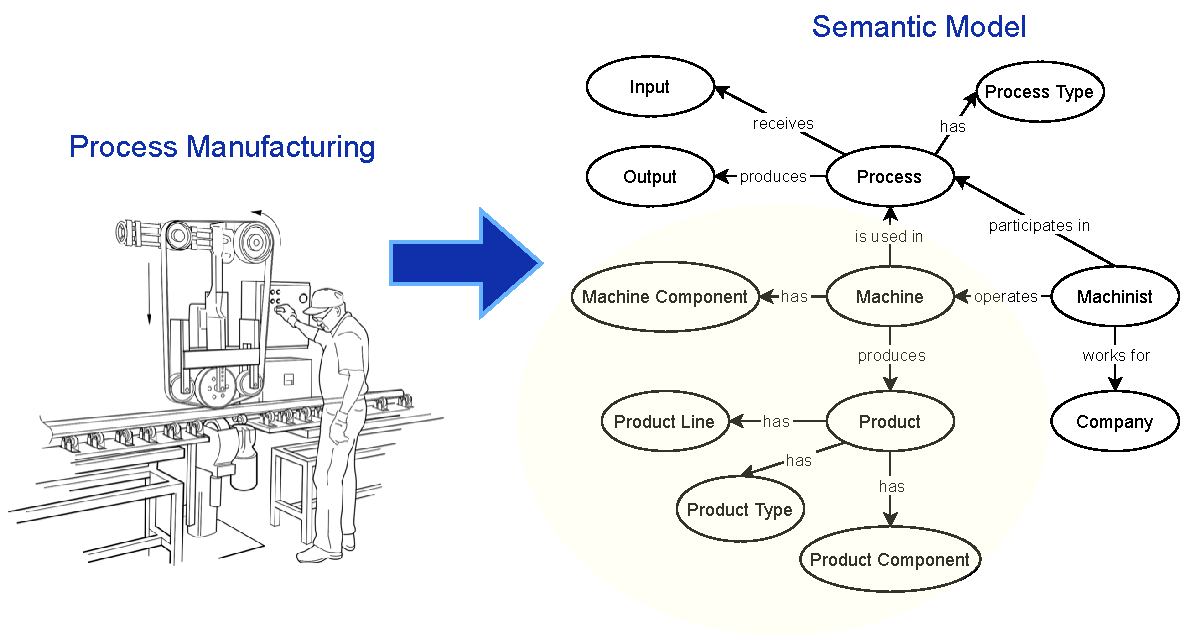
\includegraphics[width=1\textwidth,]{images/semanticmodel.pdf}
    \caption{A semantic model as an abstraction of the concepts related to the manufacturing domain}
     \label{fig:semanticmodelexample}
\end{figure}

    
In the example in Fig. \textbf{\ref{fig:semanticmodelexample}}, we present a subset of this semantic model representing some concepts, also called classes of the manufacturing domain, in which we describe the following classes \textcolor{blue}{\textbf{Product, Product Line, Price, Machine, Machine Component}} and \textcolor{blue}{\textbf{Company}}. \singlespacing

Each class has a set of properties. For instance, the class \textcolor{blue}{\textbf{Machine}} has the following properties: \textcolor{arsenic}{\textbf{\textit{id, serial number, name, fabrication date, maintenance date}}}. Additionally, every two classes relate to each other through specific relations. Here we focus on two classes: \textcolor{blue}{\textbf{Machine}} and \textcolor{blue}{\textbf{Product}}. \singlespacing

\newpage

\textcolor{blue}{\textbf{Machine}} is linked to \textcolor{blue}{\textbf{MachineComponent}} through the relation \textcolor{phthalogreen}{\textbf{\textit{hasMachineComponent}}}, then it can be expressed that
    \begin{figure}[H]
        \centering
          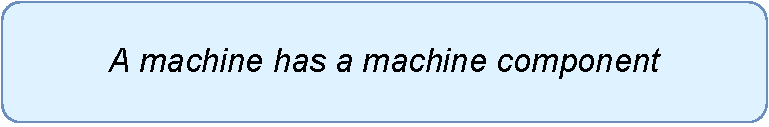
\includegraphics[width=0.5\textwidth]{images/implications0.pdf}
    \end{figure}

Also, \textcolor{blue}{\textbf{Machine}} is connected to \textcolor{blue}{\textbf{Product}} through the relation \textcolor{phthalogreen}{\textbf{\textit{isProducedBy}}}. Then we know that:

    \begin{figure}[H]
        \centering
        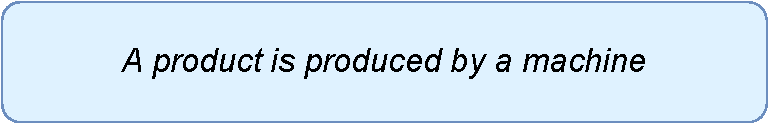
\includegraphics[width=0.5\textwidth]{images/implications0-2.pdf}
    \end{figure}
    
If we contrast both semantic models presented in Figures \textbf{\ref{fig:semanticmodelprocess}} and \textbf{\ref{fig:semanticmodelexample}} we can notice, for instance, that the relation between \textcolor{blue}{\textbf{Machine}} and \textcolor{blue}{\textbf{Product}} is expressed differently. In the first example the relation is called \textcolor{phthalogreen}{\textbf{\textit{produces}}} and it goes from \textcolor{blue}{\textbf{Machine}} to \textcolor{blue}{\textbf{Product}}, while in the second example it goes from \textcolor{blue}{\textbf{Product}} to \textcolor{blue}{\textbf{Machine}} and its called \textcolor{phthalogreen}{\textbf{\textit{isProducedBy}}}. As we can see, it is an inverse relation expressing the same information. We want to achieve this kind of expressivity through a formal model, which can also help in inferring implicit knowledge. Therefore we need ontologies, which are then core components of semantic models. \singlespacing

\begin{beware}[Note]
One should notice there is a difference between syntax and semantics when representing knowledge. We will see in the following sections, especially in \textbf{\ref{sec:semanticmodels}}, how semantics add meanings on top of a structural model.
\end{beware}

\begin{beware}[Remark]
Semantic Web Technologies, which are standards defined by the \ac{W3C} are used to represent knowledge as semantic models. The main reason to use these standards, in our domain of interest is that, as reported in \cite{Kharlamov18}, they provide an effective semantic modelling solution to data integration and industrial diagnostics serving as an abstraction of industrial assets.
\end{beware}

%%%%%%%%%%%%%%%%%%%%%%%%%%%%%%%%%%%%%%%%%%%%%%%%%%%
%% Ontologies
%%%%%%%%%%%%%%%%%%%%%%%%%%%%%%%%%%%%%%%%%%%%%%%%%%%

\subsection{Ontologies}
\label{sec:ontologies}
Even though the term \textit{Ontology} has its origins in Philosophy, it is a well-known concept in the field of Knowledge Engineering and Information Science \cite{Peng13}. A short definition given by Gruber \cite{Gruber93} is that ``an ontology is a specification of a conceptualisation" and usually follows a hierarchy of the described concepts \cite{Kalfoglou05}. In another definition, ontologies are an explicit and formal description of terms in a given domain, the properties or roles of those concepts, and the existent restrictions (if they are) \cite{Noy01,Peng13}. \singlespacing

\subsubsection{What are Classes in an Ontology}
\label{sec:classesontologies}

Classes are the important terms one wants to describe. One uses classes in ontology to group similar resources and then to have a hierarchy. Let's consider the example in Fig. \textbf{\ref{fig:exampleclasses}}. Here the classes are \textbf{Machine}, \textbf{MachineComponent}, \textbf{Component} and \textbf{PhysicalObject}, \textbf{Product}, \textbf{ProductComponent}, and \textbf{ProductLine}. 

  \begin{figure}[H]
        \centering
          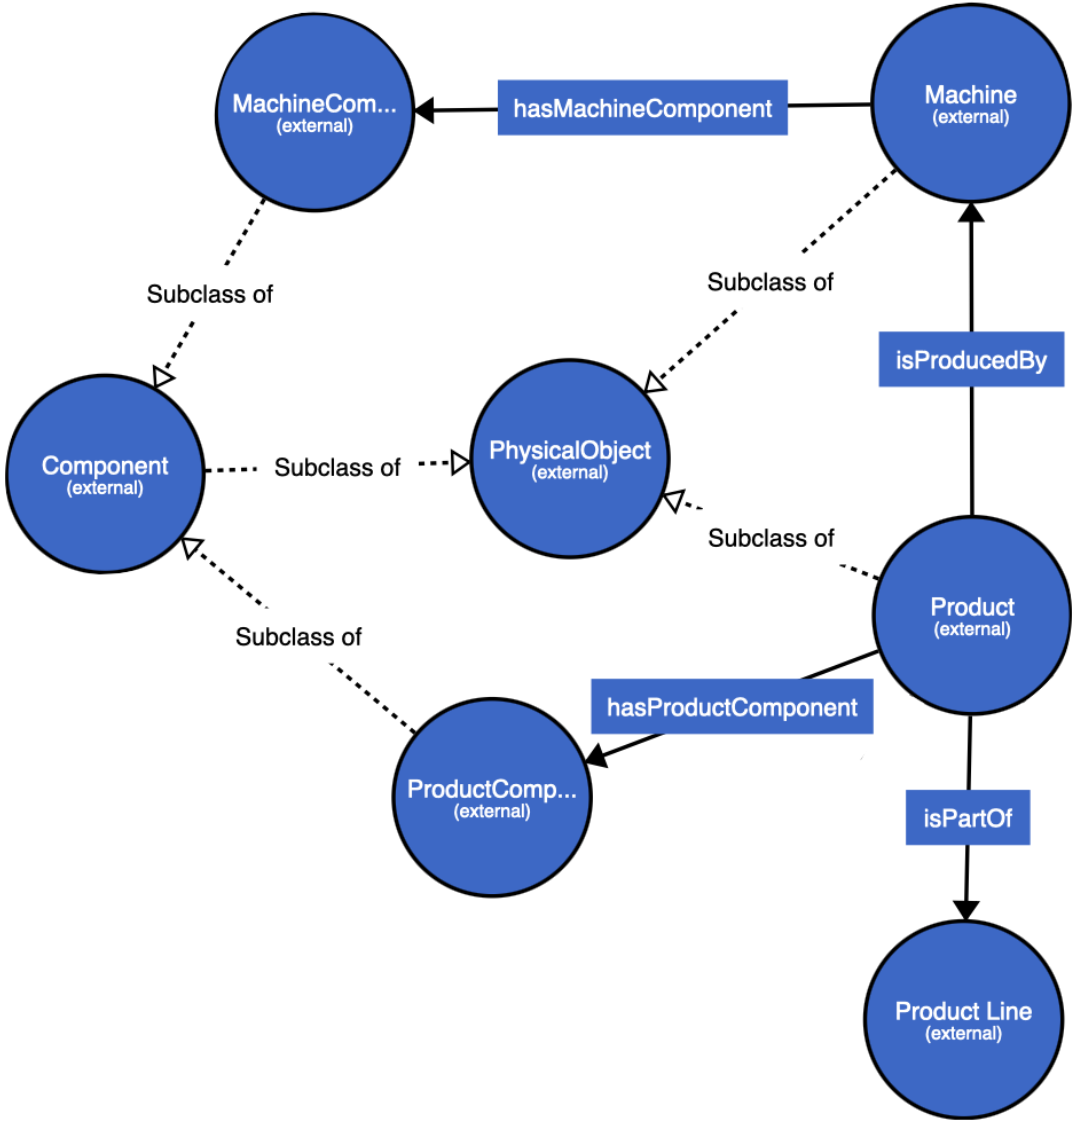
\includegraphics[width=0.6\textwidth]{images/classesexample.png}
          \caption{Examples of Classes}
    \label{fig:exampleclasses}
    \end{figure}

Here we also observe how to build a hierarchy, in this case consider:

 \begin{SampleEnv}
    \begin{figure}[H]
    \begin{mdframed}[backgroundcolor=mediumtealblue!8, linecolor=mediumtealblue]
        \begin{minipage}[t]{1\linewidth}
        A \textbf{Machine Component} is a subclass of a \textbf{Component}, and
        \\
        A \textbf{Machine} is a subclass of a \textbf{Physical Object}
        \end{minipage}
     \end{mdframed}
    \end{figure}
    \label{fig:exampleHierarchy}
    \end{SampleEnv}

\newpage
Visually, the class hierarchy is as follows:
    
  \begin{figure}[H]
        \centering
          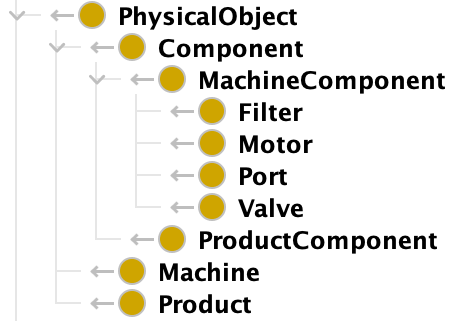
\includegraphics[width=0.6\textwidth]{images/hierarchy.png}
          \caption{Class Hierarchy}
    \label{fig:examplehiearchyclasses}
    \end{figure}

The meaning here is that a Machine Component is a more specific type of Component. In this way, one can build a hierarchy of the classes in the ontology.

\subsubsection{What are Properties in an Ontology}
\label{sec:propertiesontologies}

Properties, on the other hand are the linking attributes one wants to use to relate two classes (object properties) or a class and a value (data properties).

  \begin{figure}[H]
        \centering
          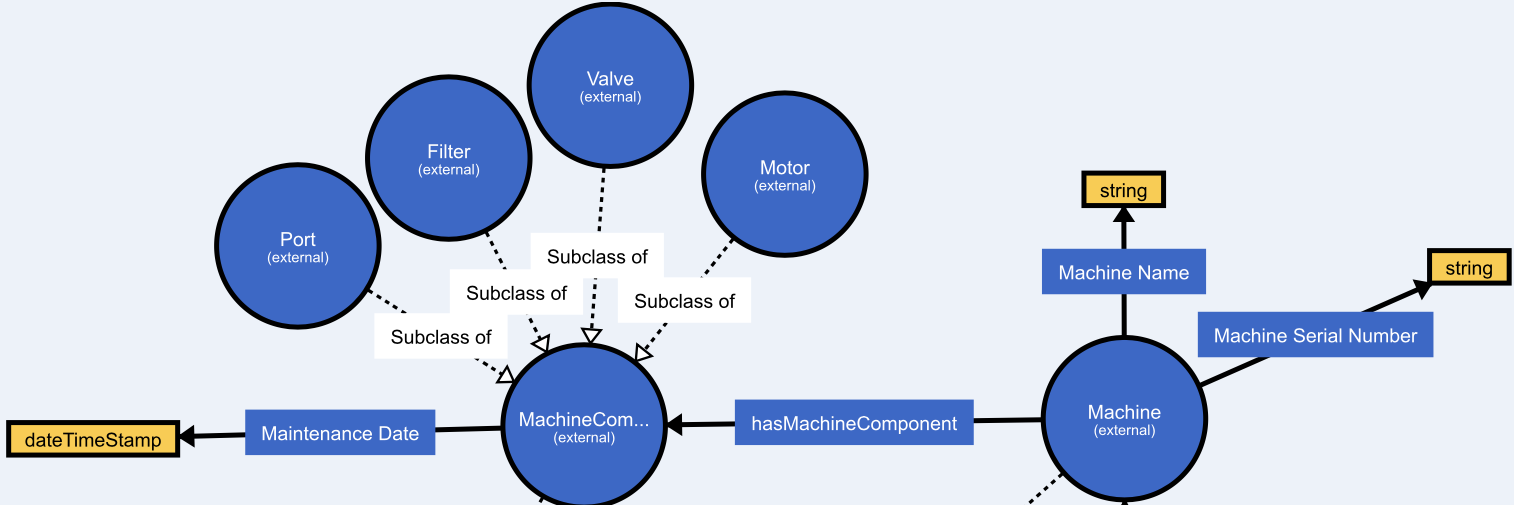
\includegraphics[width=\textwidth]{images/properties.png}
          \caption{Examples of Data and Objects Properties}
    \label{fig:exampleproperties}
    \end{figure}

Now consider Fig. \textbf{\ref{fig:exampleproperties}}, which is a subset of the ontology we present in Fig. \textbf{\ref{fig:ontologyexample}}, one property here is \textit{"hasMachineComponent"}. In this case, it is a object property as it is linking two classes in the ontology (Machine and MachineComponent).
    
 \begin{SampleEnv}
    \begin{figure}[H]
    \begin{mdframed}[backgroundcolor=mediumtealblue!8, linecolor=mediumtealblue]
        \begin{minipage}[t]{1\linewidth}
        Machine \textit{hasMachineComponent} MachineComponent
        \end{minipage}
     \end{mdframed}
    \end{figure}
    \label{fig:exampleOBJECTPropertytext}
    \end{SampleEnv}
    
\newpage
On the other hand, the property \textit{"Maintenance Date"} is a data property, as it is linking a class (MachineComponent) with a value, in this case a data of type date/time. For example, consider the following:

 \begin{SampleEnv}
    \begin{figure}[H]
    \begin{mdframed}[backgroundcolor=mediumtealblue!8, linecolor=mediumtealblue]
        \begin{minipage}[t]{1\linewidth}
        A Machine Component \textit{hasMaintenanceDate} "2017-04-12T10:30:00"
        \end{minipage}
     \end{mdframed}
    \end{figure}
    \label{fig:exampleDataPropertyText}
    \end{SampleEnv}

\subsubsection{What are Domains and Ranges in the Elements of an Ontology}
\label{sec:domainrangeontologies}

The domain is the class that is the subject of what we are describing by using that property, and the range is the object. In other words, they better indicate the relation between the elements that use a specific property and allow inference. \singlespacing

Following the previous examples, consider Fig. \textbf{\ref{fig:domainrangeobjectproperty}}. In this case, we can see that the domain of the property is \textbf{Machine}, and the range is \textbf{MachineComponent}. The meaning of such modelling is that a Machine has a machine component, or say differently, that a machine component belongs to a machine.

  \begin{figure}[H]
        \centering
          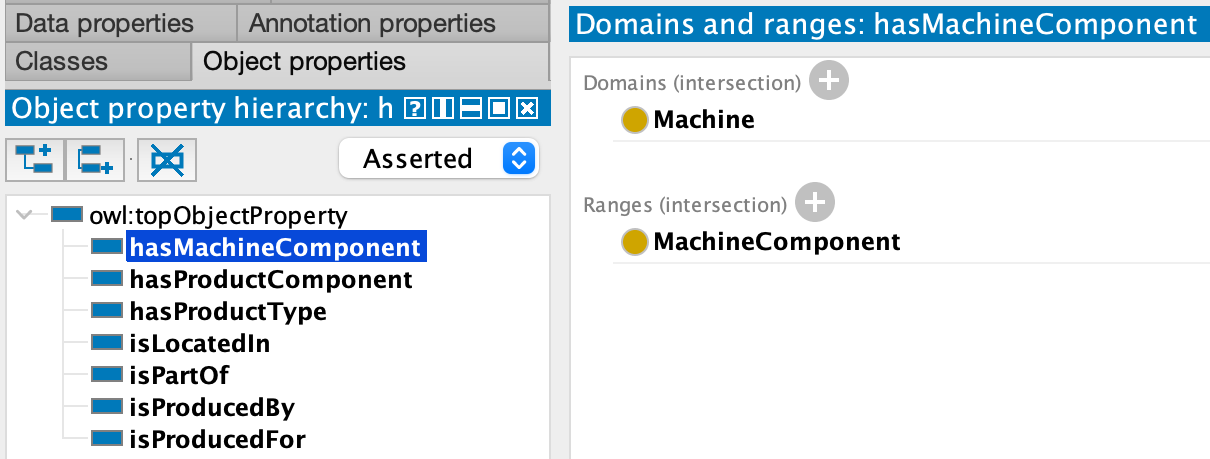
\includegraphics[width=\textwidth]{images/domainrange.png}
          \caption{Examples of Domain and Range in an Object Property}
    \label{fig:domainrangeobjectproperty}
    \end{figure}
    
In the case of a data property, consider again the example "Maintenance Date". We said, it is a data property, and as we see in Fig. \textbf{\ref{fig:domainrangedataproperty}}, the domain now is a class (MachineComponent), but the range is a value, in this case of type datetime. Then, this modelling is expressing that a component of a machine undergoes maintenance on a given date.

 \begin{figure}[H]
        \centering
          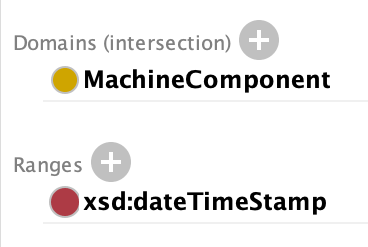
\includegraphics[width=0.5\textwidth]{images/domainrangedataproperty.png}
          \caption{Examples of Domain and Range in a Data Property}
    \label{fig:domainrangedataproperty}
    \end{figure}


Also, let's consider the following piece of knowledge:
 \begin{SampleEnv}
    \begin{figure}[H]
    \begin{mdframed}[backgroundcolor=mediumtealblue!8, linecolor=mediumtealblue]
        \begin{minipage}[t]{1\linewidth}
        A Product is made of Polyethylene terephthalate (PET)
    \end{minipage}
     \end{mdframed}
    \end{figure}
    \label{fig:exampleDomainRange}
    \end{SampleEnv}

Here, the property would be \textit{"isMadeOf"}, while \textbf{PET} and \textbf{PETBottle} are the classes. Now, by looking at the structure of the sentence we are using to express some knowledge, we see that \textbf{PETBottle} is the subject of the sentence, \textit{isMadeOf} is the predicate, and \textbf{PET} is the object. \singlespacing

Likewise, we can say that the \textbf{domain} (subject), then is \textbf{PETBottle}, and the \textbf{range} (object) is \textbf{PET}.


\subsubsection{What are Individuals in an Ontology}
\label{sec:individualsontologies}

One can associate each class with a set of individuals. The individuals in the class are called the instances of the class and they are the most specialised or specific concepts one wants to model. \singlespacing

 \begin{SampleEnv}
    \begin{figure}[H]
    \begin{mdframed}[backgroundcolor=mediumtealblue!8, linecolor=mediumtealblue]
        \begin{minipage}[t]{1\linewidth}
        A PET bottle is produced by an Injection Blow Moulding Machine
    \end{minipage}
     \end{mdframed}
    \end{figure}
    \label{fig:exampleIndividuals}
    \end{SampleEnv}
    
Here, PET bottle is an instance of the class Product, and Injection Blow Moulding Machine is an instance of the class Machine. \singlespacing


To illustrate the above-given definitions, we present an example in Fig. \textbf{\ref{fig:ontologyexample}} in a graph form, in which we follow the previously introduced examples. Here we can notice two types of relationships between concepts. One of these types expresses hierarchical relations by indicating that a class is a subclass of (\textbf{\textit{SubclassOf}}) another one. The other expresses the specific connection between concepts, for instance \textcolor{phthalogreen}{\textbf{\textit{isProducedBy}}} and \textcolor{phthalogreen}{\textbf{\textit{hasMachineComponent}}}.
    
    \begin{figure}[H]
        \centering
          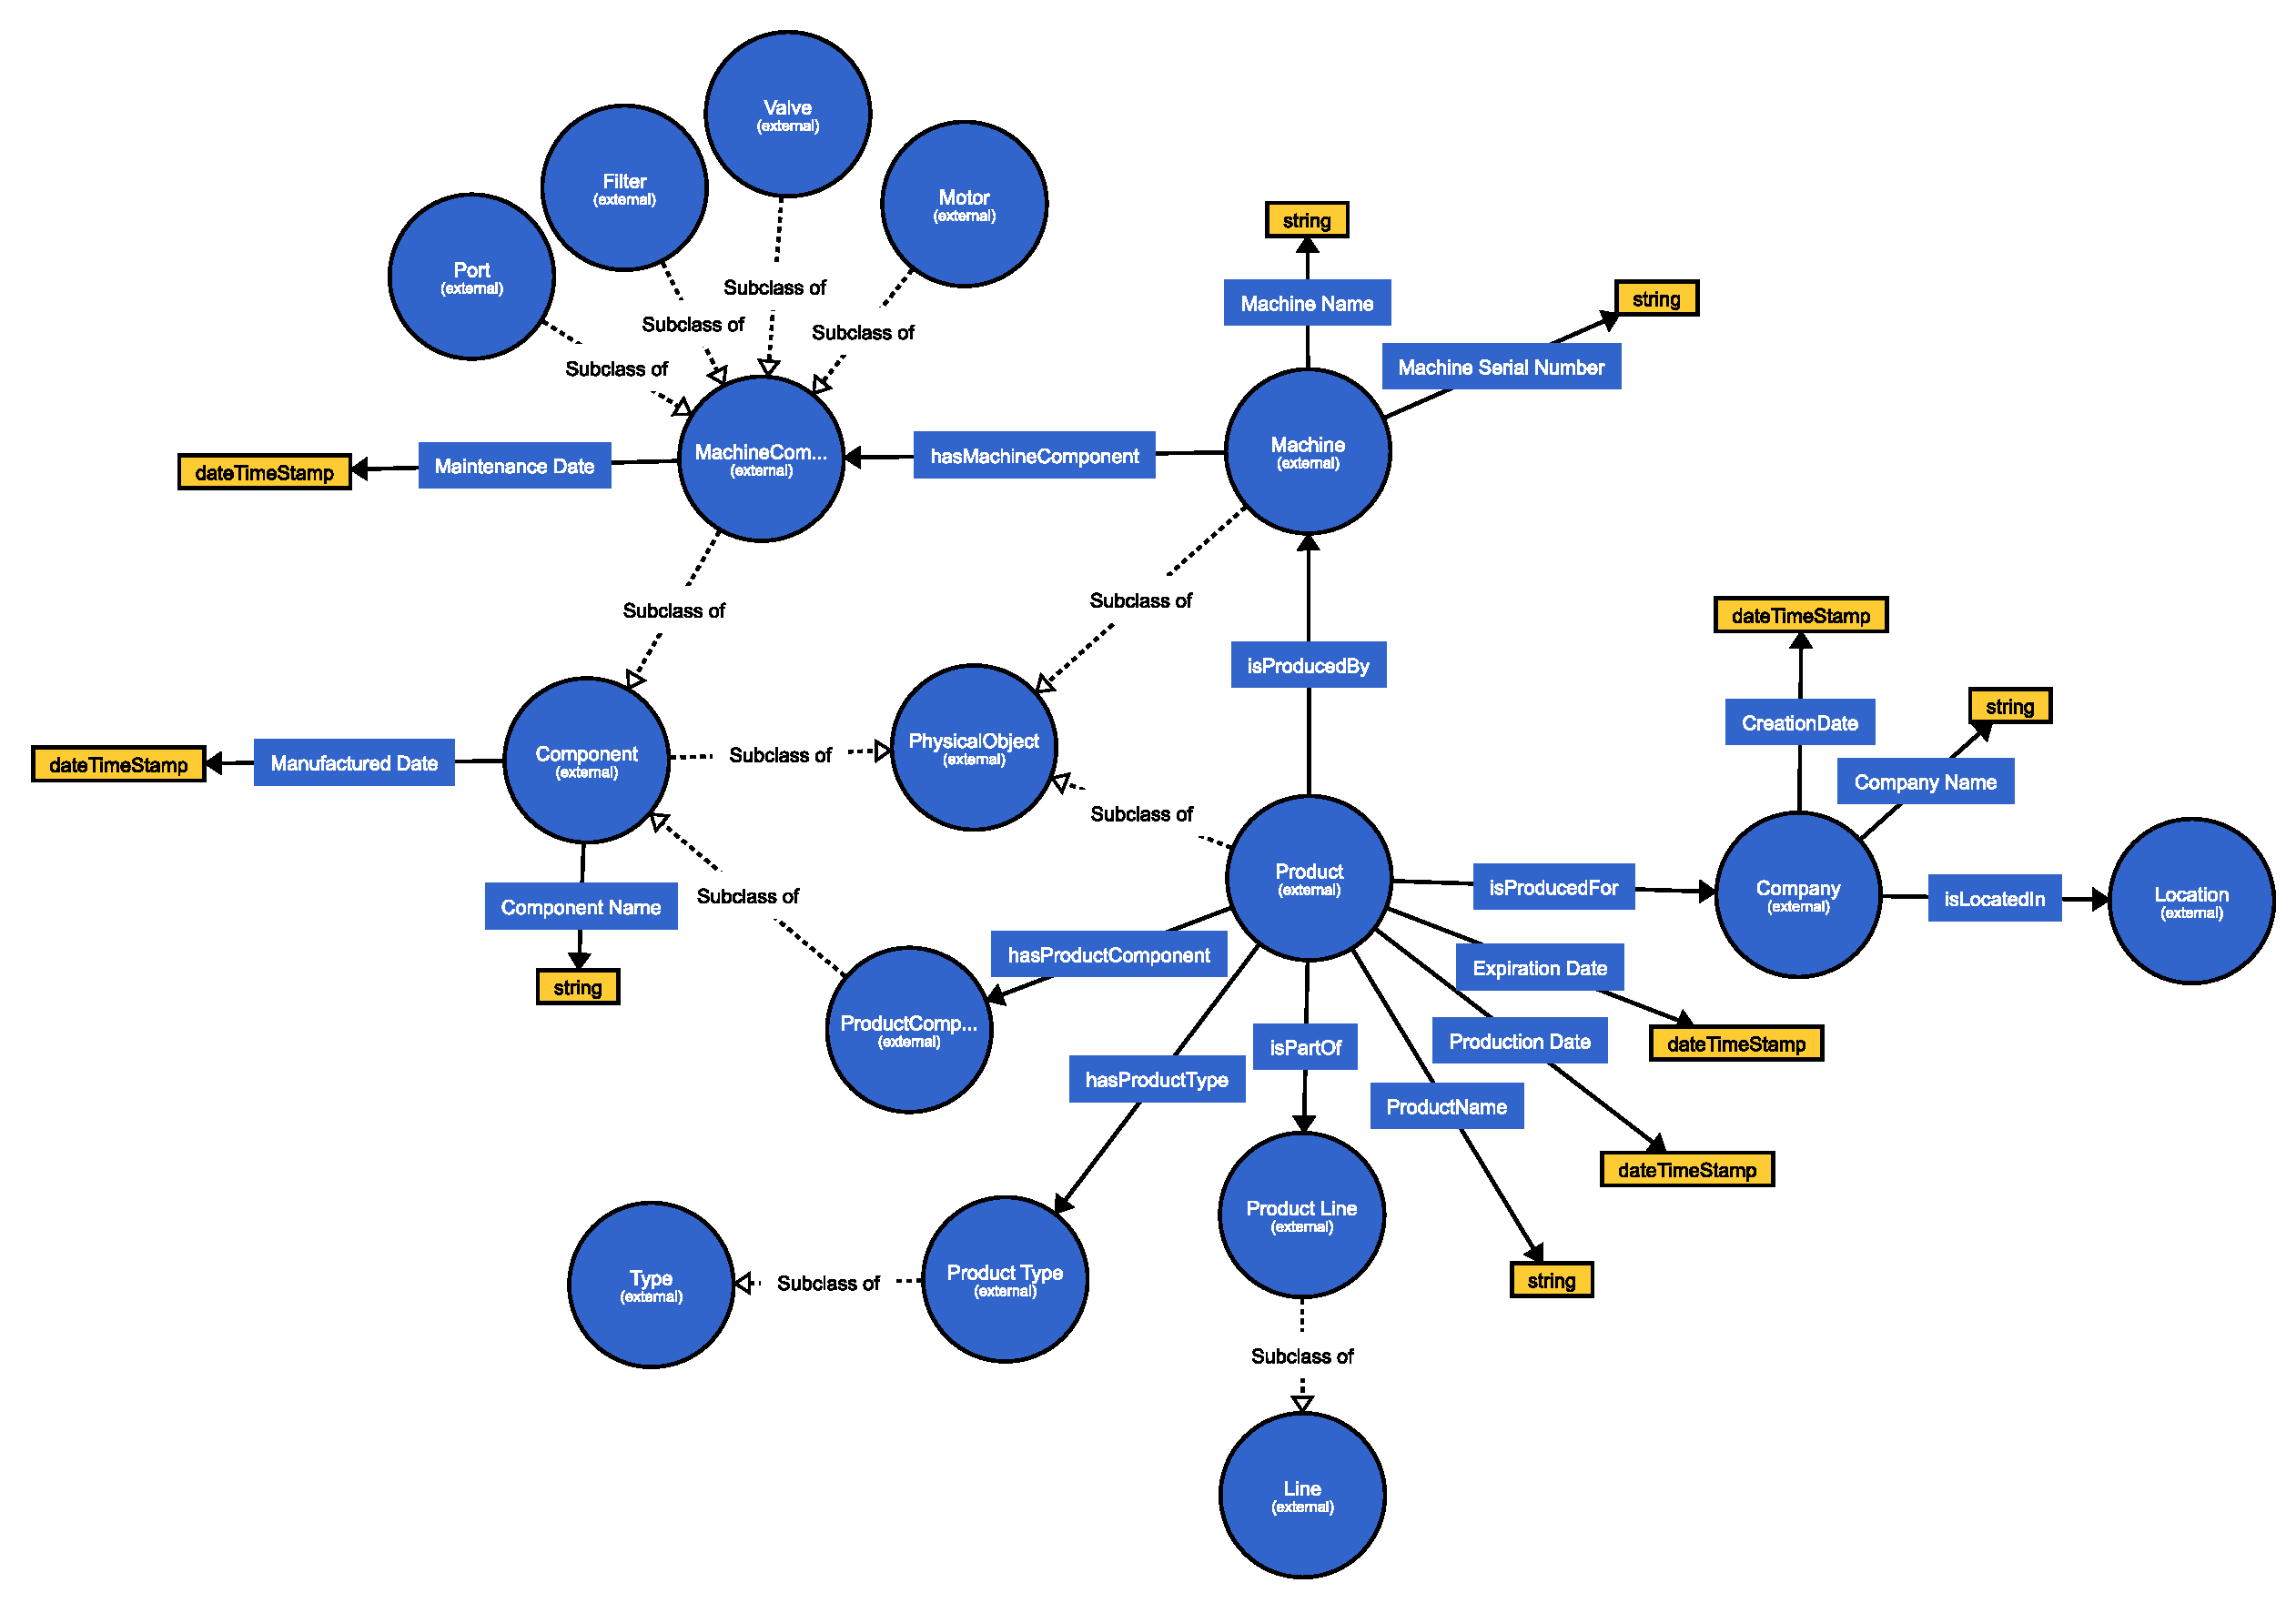
\includegraphics[width=1\linewidth]{images/example-ontology.pdf}
          \caption{An ontology representing a subset of knowledge related to the manufacturing domain by definition of concepts and their relationships}
        \label{fig:ontologyexample}
    \end{figure}

\begin{beware}[Note]
We used the WebVOWL tool to generate the graphical representation of the small ontology presented in Fig. \textbf{\ref{fig:ontologyexample}}. We introduce WebVOWL in Chapter \textbf{\ref{sec:tools}}.
\end{beware}  \singlespacing

By following the example in Fig. \textbf{\ref{fig:semanticmodelexample}}, we can observe how the ontology in Fig. \textbf{\ref{fig:ontologyexample}} also includes the representation of that knowledge. Now if we focus again on the relations \textcolor{phthalogreen}{\textbf{\textit{isProducedBy}}} and \textcolor{phthalogreen}{\textbf{\textit{hasMachineComponent}}} between the classes \textcolor{blue}{\textbf{Product}} and \textcolor{blue}{\textbf{Machine}}, and \textcolor{blue}{\textbf{Machine}} and \textcolor{blue}{\textbf{MachineComponent}} respectively, we can say that the same might be expressed by the inverse relations \textcolor{phthalogreen}{\textbf{\textit{produces}}} and  \textcolor{phthalogreen}{\textbf{\textit{belongsTo}}}. It is possible to reach this kind of conclusion by applying inference tools to an ontology. Then it is possible to infer the following knowledge from the ontology: \\

    \begin{figure}[H]
        \centering
          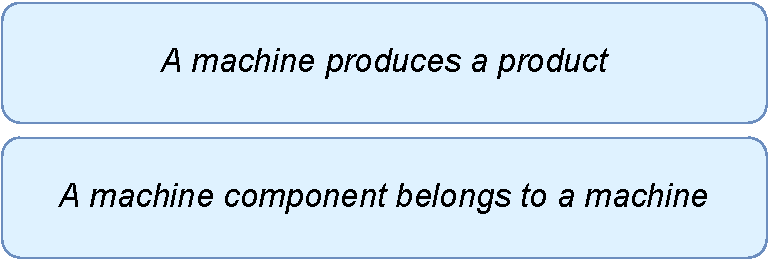
\includegraphics[width=0.5\textwidth]{images/implications1.pdf}
    \end{figure}

\newpage
In this context, we need to remark that when modelling ontologies, it is essential to consider the concepts of \ac{CWA} and \ac{OWA}. \ac{CWA} assumes complete information, i.e., it is the assumption that what is not known to be \colorbox{junglegreen!50}{\texttt{True}} is \colorbox{pastelred!50}{\texttt{False}} \cite{Keet13-2}. On the other hand, \ac{OWA} is the assumption that anything that is not known (to be true or false) is considered \textit{unknown}, but not false \cite{Ramis21}. Therefore, it assumes incomplete information \cite{Keet13-1}, and the distinction between something being \colorbox{pastelred!50}{\texttt{False}} and something being \colorbox{bananamania}{\texttt{Unknown}} is possible \cite{Uschold15}. \singlespacing

We can argue that it is possible to infer knowledge from the ontology without the higher complexity needed in the \ac{ER} model to achieve similar results. In other words, it is possible to join several tables in a database (corresponding to the \ac{ER} model) to get similar knowledge provided by ontologies, but it requires more effort. The reason is that ontologies add semantics by explicitly defining relations between classes, and in this way, allowing interoperability and more expressiveness \cite{Ramis21}. Moreover, the main difference between \ac{ER} models and ontologies is that while the former uses \ac{CWA} and adds constraints, the latter benefits from \ac{OWA}. In this context, there are some considerations, such as those presented in \cite{Uschold15}, to take into account when considering \ac{CWA} or \ac{OWA} for inferring knowledge. \singlespacing

To clarify the concepts of \ac{CWA} and \ac{OWA}, let's look at the two main differences between them when it comes to answering direct questions and inferring new knowledge \cite{Sequeda12}. For this, we will consider Fig. \textbf{\ref{fig:examplesCWAOWA}}, where we show a subset of the ontology introduced in Example \textbf{\ref{fig:ontologyexample}}, and assume the following facts (axioms) are part of the model in our ontology and in a relational database: \singlespacing

\begin{mdframed}[backgroundcolor=arsenic!8, linecolor=arsenic]
\begin{minipage}[t]{1\linewidth}
  \begin{enumerate}
    \item A PET bottle is a product \label{ax:1}
    \item A PET bottle is made of PET \label{ax:2}
    \item PET is a recyclable plastic \label{ax:3}
     \item HDPE is a recyclable plastic \label{ax:4}
    \item A product is produced only by one machine \label{ax:5}
    \item An extrusion blow moulding machine is a machine \label{ax:6}
    \item An injection blow moulding machine is a machine \label{ax:7}
    \item A PET bottle is produced by an injection blow moulding machine \label{ax:8}
    \item A machine component is a component \label{ax:9}
    \item A component is a physical object \label{ax:10}
   %\item A product can have several product lines
   %\item A PET Bottle has product line ``Water Bottle"
   %\item A PET Bottle has product line ``Vegetable Oil Container"
    \item Anything that is made of recyclable plastic is recyclable \label{ax:11}
  \end{enumerate}
\end{minipage}
\end{mdframed}

\begin{figure}[H]
    \begin{minipage}{\textwidth}
            \centering
         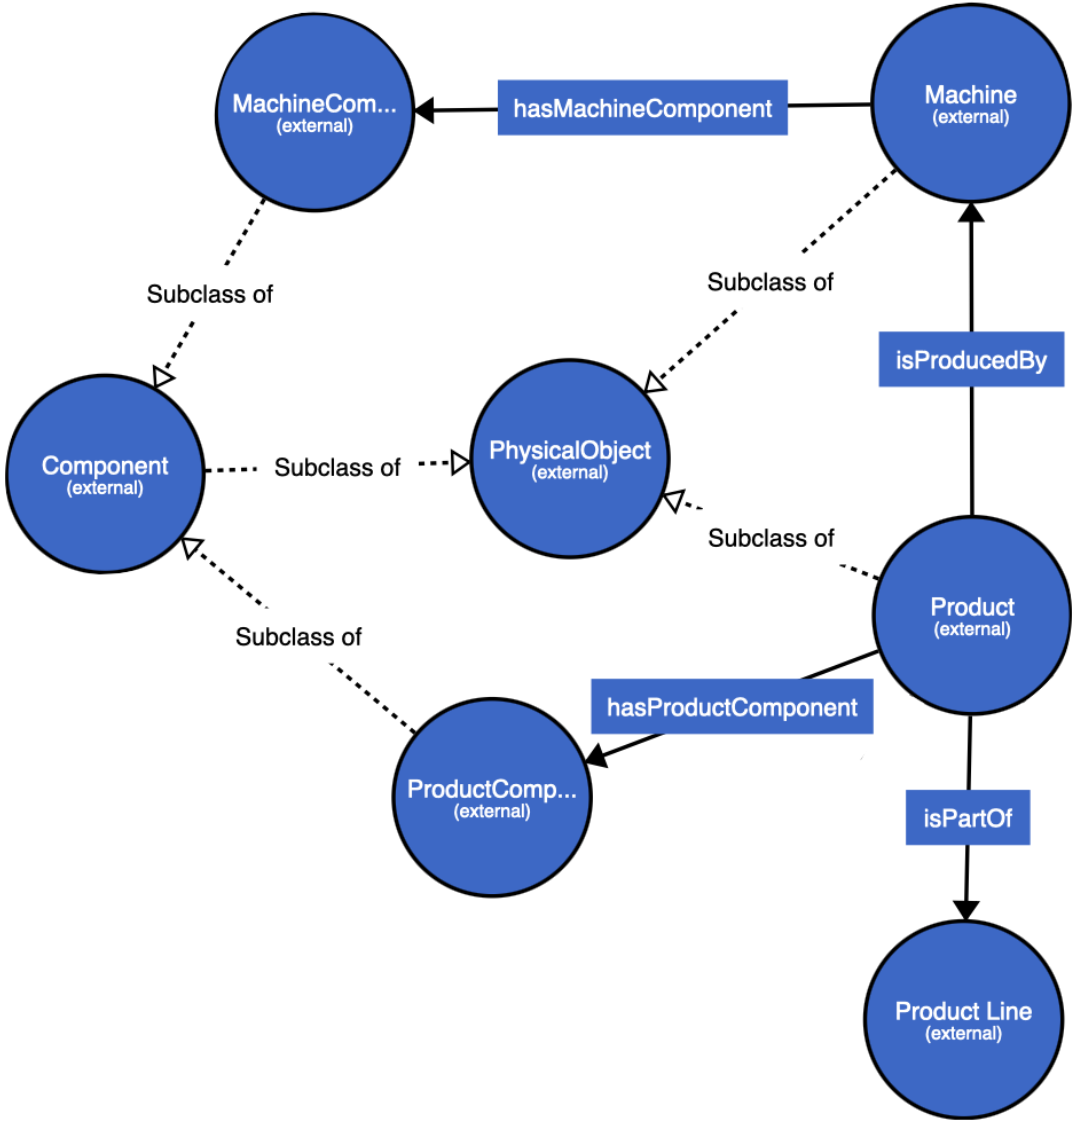
\includegraphics[width=0.6\textwidth]{images/examplesCWAOWA.png}
    \end{minipage}%
    \caption{Subset of the Ontology presented in Example \textbf{\ref{fig:ontologyexample}}} \label{fig:examplesCWAOWA}
\end{figure}

Regarding answering direct questions, consider we ask  \colorbox{arsenic!20}{\texttt{"Is there a product called PET bottle?"}}. The answer in both, relational databases (considering the \ac{CWA}) and ontology (considering the \ac{OWA}) will be \colorbox{junglegreen!50}{\texttt{"Yes"}} because such query will return the answer \colorbox{junglegreen!50}{\texttt{True}} considering the fact \textbf{\ref{ax:1}}. When we ask \colorbox{arsenic!20}{\texttt{"Are PET and HDPE recyclable plastics?"}}, we will again get the answer \colorbox{junglegreen!50}{\texttt{"Yes"}}, as it is possible to answer this question directly by the facts \textbf{\ref{ax:3}} and \textbf{\ref{ax:4}}. However, if we now ask \colorbox{arsenic!20}{\texttt{"Is there a product called PP bottle?"}}, we expect to get the answer \colorbox{pastelred!50}{\texttt{"No"}} in relational databases because there is no information about such a product in our model (defined facts). That would be the case because the associated query will return \colorbox{pastelred!50}{\texttt{False}}. On the other hand, in the ontology, instead of getting the answer \colorbox{pastelred!50}{\texttt{"No"}}, we expect to get the answer \colorbox{bananamania}{\texttt{"Unknown"}}. That is the correct behaviour in this scenario because the ontology would need more facts to disprove the assumption that such a product exists, i.e., to demonstrate that a product with that name does not exist, as it assumes the \ac{OWA}. 
\singlespacing

Next, suppose we ask \colorbox{arsenic!20}{\texttt{"Is a machine component a physical object?"}}. In the ontology (\ac{OWA}), the answer will be \colorbox{junglegreen!50}{\texttt{"Yes"}}, and as shown in Example \textbf{\ref{fig:exampleMachineComponent}}, the explanation will result from the transitivity property of the relations between concepts, i.e., as a Machine Component is a subclass of Component (related to fact \textbf{\ref{ax:9}}), and Component is a subclass of Physical Object (related to fact \textbf{ \ref{ax:10}}), it must be the case that a Machine Component is a Physical Object. We show these relations in the example by the green arrows. Likewise, it would be possible to reach that conclusion by a query joining the corresponding tables in relational databases, as there is no explicit meaning in the relationships.

\begin{SampleEnv}
\begin{figure}[H]
\begin{mdframed}[backgroundcolor=mediumtealblue!8, linecolor=mediumtealblue]
\noindent\begin{minipage}{1\textwidth}
        (MachineComponent subClassOf Component) \textit{AND} \\
        (Component subClassOf PhysicalObject) \textit{IMPLIES THAT} \\
        (MachineComponentsubClassOf PhysicalObject)
\end{minipage}
\noindent\begin{minipage}{1\textwidth}
\centering
  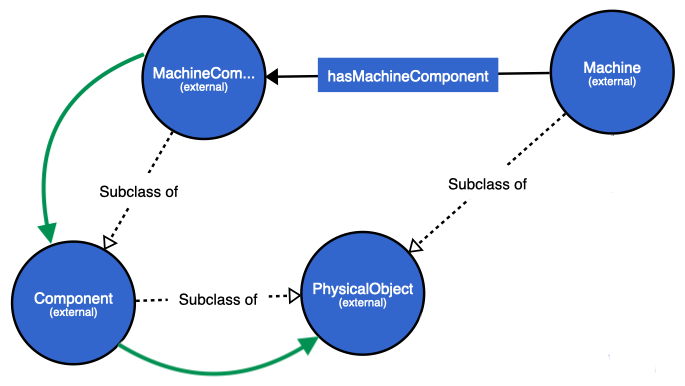
\includegraphics[width=0.6\textwidth]{images/transitivityExampleInference.png}
\end{minipage}
 \end{mdframed}
\end{figure}
\label{fig:exampleMachineComponent}
\end{SampleEnv}

Now, regarding knowledge inference capabilities of an ontology, consider our model under the facts expressed by facts \textbf{\ref{ax:5}} and \textbf{\ref{ax:8}}. If we want to add a new fact  \colorbox{arsenic!10}{\textit{``A PET bottle is produced by an extrusion blow moulding machine"}}, we would get two different scenarios, depending on if we consider the \ac{CWA} or the \ac{OWA}, as we describe below. \singlespacing

In the \ac{CWA} as soon as we want to add the new fact, we would get an error by contradiction to our initial assumption that a product is produced only by one machine (fact \textbf{\ref{ax:5}}). \singlespacing
    
On the contrary, in the \ac{OWA} instead of an error, this new statement would let the ontology infer a piece of new knowledge. That is, \colorbox{magicmint!10}{\texttt{"if a product is produced only by one machine, and if PET bottle is produced by}} \colorbox{magicmint!10}{\texttt{an injection blow moulding machine and an extrusion blow moulding machine, then}} \colorbox{magicmint!10}{\texttt{injection blow moulding machine and extrusion blow moulding machine must be}} \colorbox{magicmint!10}{\texttt{referring to the same concept"}}. The ontology reaches such a conclusion because the de facto language for ontology creation, \ac{OWL}, does not make the \ac{UNA}\footnote{The Unique Name Assumption indicates that different names always refer to different entities in the world \cite{Russell16}}. Thus, to avoid such behaviour, one should explicitly state that two resources with distinct \ac{URI}s \footnote{An \ac{URI} is a unique identifier that enables uniform identification of logical and physical resources \cite{RFC3986}} are different. \singlespacing

    
Now consider we ask: \colorbox{arsenic!20}{\texttt{"Is PET bottle recyclable?"}} The answer in the relational database and the ontology would be \colorbox{junglegreen!50}{\texttt{"Yes"}} by the inference that is a PET Bottle is made of PET and PET is a recyclable plastic, then PET Bottle must be also a recyclable plastic. \singlespacing

However, if we ask \colorbox{arsenic!20}{\texttt{"Is HDPE bottle recyclable?"}} in a relational database, the answer would be \colorbox{pastelred!50}{\texttt{"No"}} because there is no information in the list of facts indicating such knowledge. On the other hand, in an ontology, the answer, by fact \textbf{\ref{ax:11}}, would be that there could be a model satisfying such conclusion, for example, by adding a new fact  \colorbox{arsenic!10}{\textit{``HDPE bottle is made of HDPE"}}. Because we know, by fact \textbf{\ref{ax:4}} that HDPE is a recyclable plastic and anything made of recyclable plastic is recyclable.

\subsection{Classification of Ontologies} \label{sec:classificationontologies}

An important consideration regarding ontologies is that they are classified depending on their coverage. Here, we describe the following: \singlespacing

\begin{itemize}
    \item \textcolor{sapphire}{\textbf{Upper Ontologies:}} also called ``Top-Level" ontologies, are highly generic and represent the concepts, categories and relations common to various domains.
    \item \textcolor{sapphire}{\textbf{Domain Ontologies:}} they represent concepts related to a specific domain, such as objects, tasks, activities, and processes in that domain.
    \item \textcolor{sapphire}{\textbf{New Ontology:}} refers to the new ontology one is currently creating to model a specific use case.
    \item \textcolor{sapphire}{\textbf{Support Ontologies:}} are the ontologies that can be used cross-sectionally, i.e., across different domains, for example to express organizational structures.
\end{itemize} \singlespacing

In Fig. \textbf{\ref{fig:ontologycomposition}} we illustrate the different ontology levels relevant for creating reusable and interoperable ontologies in our domain of interest. Upper ontologies are at the bottom of the figure, depicting that this type of ontologies is the base of the ontology construction system. Then, on top of that, one adds middle or domain ontologies. Finally, one adds the concepts of the new ontology. At the same time, supporting ontologies, which represent cross-domain concepts, should be considered. This representation means that one should reuse as much as possible the already defined concepts from other ontologies and newly define those specific for the use case one is modelling.

    \begin{figure}[H]
        \centering
          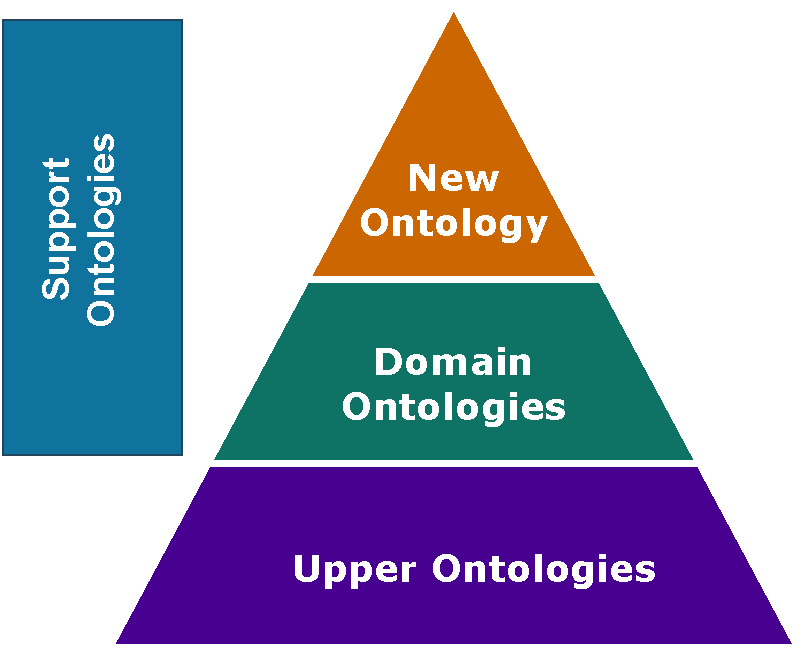
\includegraphics[width=0.5\textwidth]{images/OntologyComposition.pdf}
          \caption{Ontology Composition}
    \label{fig:ontologycomposition}
    \end{figure}

    
\begin{beware}[Remark]
It is crucial to consider reusing existing ontologies to ensure interoperability among ontologies. Therefore, it is relevant to understand their coverage and when to reuse them.
\end{beware}


\newpage
\subsection{Ontology Development Process}

To start the ontology development process, we first choose a methodology and adequate tools for the tasks at hand and adopt the best practices to tackle this task.\singlespacing

In Fig. \textbf{\ref{fig:stepsNoy}}, we show the most common steps to follow in the process, after choosing the methodology to follow and the tools to use.

    \begin{figure}[H]
        \centering
          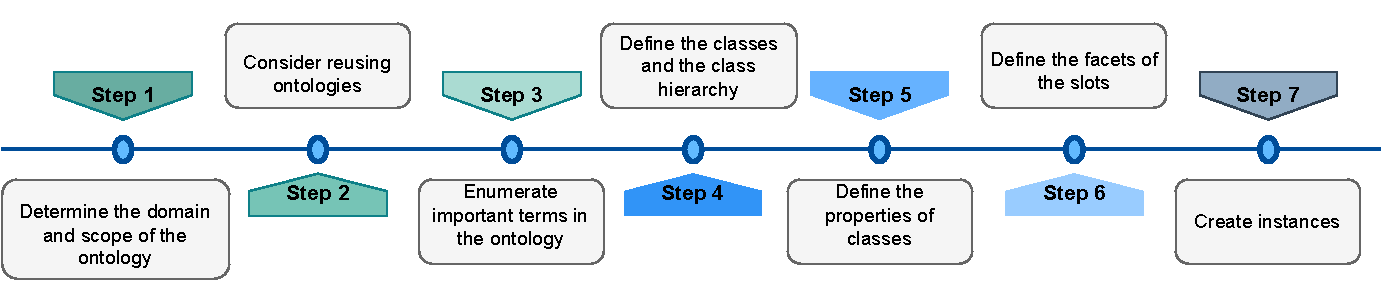
\includegraphics[width=1\linewidth]{images/StepsNoy.pdf}
          \caption{Iterative steps required to develop an ontology, based on \cite{Noy01}}
        \label{fig:stepsNoy}
    \end{figure}
    
%%%%%%%%%%%%%%%%%%%%%%%%%%%%%%%%%%%%%%%%%%%%%%%%%%%
%% Methodologies
%%%%%%%%%%%%%%%%%%%%%%%%%%%%%%%%%%%%%%%%%%%%%%%%%%%
\section{Methodologies}
\label{sec:methodologies}
There are several methodologies for ontology development, and as we explained in Chapter \textbf{\ref{sec:Introduction}}, one of the current problems in building an ontology is selecting an adequate methodology. Even though the steps presented in Fig. \textbf{\ref{fig:stepsNoy}} are relevant to start building an ontology, a more comprehensive methodology is necessary.  \singlespacing

\subsection{Recommended Ontology Development Methodology}

We recommend using the \textbf{Linked Open Terms (LOT)} methodology introduced in \cite{Poveda22}, which is available at:
\url{https://lot.linkeddata.es}. We recommend it because it is a reasonably comprehensive methodology, and as it is an evolving approach, it covers several aspects to consider during the \ac{OntoDevProcess}. The methodology focuses on engineering aspects and offers valuable insights to engineers from different domains. Moreover, it recommends tools and best practices and covers the whole \ac{OntoDevProcess} including the later stages, namely the evaluation, documentation and maintenance of the ontology. \singlespacing

The detailed documentation of the LOT methodology is available here:  \href{https://www.sciencedirect.com/science/article/pii/S0952197622000525?via\%3Dihub}{LOT: An industrial-oriented ontology engineering framework}. Moreover, in the Appendix, in Section \textbf{\ref{sec:lotfigure}} we show the original LOT methodology views, defined by \cite{Poveda22}.

\subsection{Workflow for the Ontology Development Process}
For the creation and maintenance of ontologies, we recommend following the workflow presented in Fig. \textbf{\ref{fig:workflowsuggestion}} for the creation and maintenance of the ontology, which covers the stages of the LOT methodology. \singlespacing

\begin{beware}[Remark]
We recommend to schedule an initial meeting between \ac{DEs} and \ac{KEs} before starting the Ontology Development Process to clarify ideas and expectations.
\end{beware}

\begin{beware}[Remark]
When following the steps of the workflow, follow the best practices we name in Section \textbf{\ref{sec:bestpractices}} and the additional resources from Section \textbf{\ref{sec:additionalresources}}.
\end{beware}

\subsubsection{Description of Each Step in the Workflow}
\begin{enumerate}
\item \textcolor{sapphire}{\textbf{Identify and specify the use case:}} start the process by identifying and defining the use case for which you want to build the ontology. \label{step1}

\textbf{Answer the questions:}
\begin{itemize}
    \item What is the name of the use case? 
    \item What is this use case about? 
\end{itemize}

\begin{mdframed}[backgroundcolor=officegreen!8, linecolor=officegreen]
    \begin{minipage}[t]{1\linewidth}
     \textbf{Hint:}
      Use the template \href{https://docs.google.com/document/d/1mkHccxvvGbj3omXubZ_EbM_l7m8LfalJ/edit}{\textit{Template\_OntologyRequirementsSpecification}} provided in Section \textbf{\ref{sec:templates}}.
    \end{minipage}
\end{mdframed}

\item \textcolor{sapphire}{\textbf{Identify and define scope and purpose:}} determine the scope and purpose of the use case and the corresponding ontology. \label{step2}

\textbf{Answer the questions:} 
\begin{itemize}
    \item What are the goals of this use case? 
    \item What is the benefit of using ontologies for my use case?
    \item Who will use this ontology and use case? 
    \item Who is responsible for defining the requirements of this use case?
\end{itemize}


\begin{mdframed}[backgroundcolor=officegreen!8, linecolor=officegreen]
    \begin{minipage}[t]{1\linewidth}
    \textbf{Hint:}
      Use the template \href{https://docs.google.com/document/d/1mkHccxvvGbj3omXubZ_EbM_l7m8LfalJ/edit}{\textit{Template\_OntologyRequirementsSpecification}} \\ together with \href{https://docs.google.com/spreadsheets/d/1UwT7DnW3pIkDKmfn1jgONsp2BbiQZ4mJeeg0lOBV0DQ/edit#gid=0}{\textit{Template\_CompetencyQuestions\_Definition}} provided in Section \textbf{\ref{sec:templates}}.
    \end{minipage}
\end{mdframed}


\item \textcolor{sapphire}{\textbf{Define competency questions:}} determine how the ontology will help to answer key questions. \label{step3}

\textbf{Answer the questions:} 
\begin{itemize}
    \item What are the relevant questions the ontology should answer? 
    \item What information needs to be expressed in the model to help us achieve the goals of this use case?
\end{itemize}

\begin{mdframed}[backgroundcolor=officegreen!8, linecolor=officegreen]
    \begin{minipage}[t]{1\linewidth}
    \textbf{Hint:}
      Use the template 
      \textbf{"Template\_CompetencyQuestions\_Definition"} provided in Section \textbf{\ref{sec:templates}}.
    \end{minipage}
\end{mdframed}

\item \textcolor{sapphire}{\textbf{Verify and refine competency questions:}} check the list of competency questions and evaluate their consistency and completeness. \label{step4}

\textbf{Answer the questions:} 
\begin{itemize}
    \item Did we include all the essential questions the ontology should answer? 
    \item Did we precisely formulate the questions we are interested in? 
    \item Can we improve these competency questions?
\end{itemize}

\begin{mdframed}[backgroundcolor=officegreen!8, linecolor=officegreen]
    \begin{minipage}[t]{1\linewidth}
    \textbf{Hint:}
      Use the template 
      \href{https://docs.google.com/spreadsheets/d/1UwT7DnW3pIkDKmfn1jgONsp2BbiQZ4mJeeg0lOBV0DQ/edit#gid=0}{\textit{Template\_CompetencyQuestions\_Definition}} provided in Section \textbf{\ref{sec:templates}}.
    \end{minipage}
\end{mdframed}

\begin{enumerate}
    \item If changes are necessary to the competency questions, modify and refine them on demand.
    \item If no changes are needed, go to the next step.
\end{enumerate}

\item \textcolor{sapphire}{\textbf{Conceptualize the ontology:}}  based on the terms one identifies as important for the model, define which of them are classes, properties, and individuals.  \label{step5}

\textbf{Answer the questions:} 
\begin{itemize}
    \item What are the necessary terms we need to include? 
    \item What are the constraints and considerations in this use case?
\end{itemize}

\begin{mdframed}[backgroundcolor=officegreen!8, linecolor=officegreen]
    \begin{minipage}[t]{1\linewidth}
    \textbf{Hint:}
      Consider the information we presented in Section \textbf{\ref{sec:ontologies}} about Classes, Properties, and Individuals. Use the information you included on the documents based on templates \href{https://docs.google.com/document/d/1mkHccxvvGbj3omXubZ_EbM_l7m8LfalJ/edit}{\textit{Template\_OntologyRequirementsSpecification}} and \href{https://docs.google.com/spreadsheets/d/1UwT7DnW3pIkDKmfn1jgONsp2BbiQZ4mJeeg0lOBV0DQ/edit#gid=0}{\textit{Template\_CompetencyQuestions\_Definition}} to identify the important terms you need to model in your ontology.
      Once you identified the terms, use the templates \href{https://docs.google.com/spreadsheets/d/16g3pAnE-fzbQydI0m5zkswAc83r881oBgKarQaCkGa0/edit#gid=0}{\textit{Template\_Class\_Definition}}, \href{https://docs.google.com/spreadsheets/d/1pmVIaY3WwofKMBwXdqbiCgXH5DL4rNx-ZhKlHUdZoRo/edit#gid=0}{\textit{Template\_Property\_Definition}}, and \href{https://docs.google.com/spreadsheets/d/11_twMjg6mwAQoefg4pRDqZCcsNCKwbrflg0NIkcyF1I/edit#gid=0}{\textit{Template\_Individuals\_Definition}} from Section \textbf{\ref{sec:templates}}.
    \end{minipage}
\end{mdframed}

\item \textcolor{sapphire}{\textbf{Consider reusing existing ontologies:}} once you identify the scope of the ontology and the required terms, look for information about existing ontologies covering a similar domain, and reuse them when needed. Also, consider reusing upper (top-level) ontologies. \label{step6}

\textbf{Answer the questions:} 
\begin{itemize}
    \item Is there an ontology covering our whole use case? 
    \item Is there an ontology partially covering our use case? 
\end{itemize}

\begin{mdframed}[backgroundcolor=officegreen!8, linecolor=officegreen]
    \begin{minipage}[t]{1\linewidth}
    \textbf{Hint:}
      Consider the information presented in Section \textbf{\ref{sec:architecturalsuggestions}} and identify which terms you want to model in your ontology are already included in exiting ontologies we list in Tables \textbf{\ref{tab:upperontologies}}, \textbf{\ref{tab:currentsupportontologies}}, and in Section \textbf{\ref{sec:domainontologies}}. You can look at information about ontologies in the resources we provide in Table \textbf{\ref{tab:catalogs}}.
    \end{minipage}
\end{mdframed}

\item \textcolor{sapphire}{\textbf{Formalize \ac{ORSD} and competency questions:}} with the help of the editor tool, start creating the identified classes, properties, individuals, and the necessary relationships among them. \label{step7}

\textbf{Answer the questions:} 
\begin{itemize}
    \item Did we model all the identified entities? 
    \item Did we express all the needed relationships and constraints?
\end{itemize}

\begin{mdframed}[backgroundcolor=officegreen!8, linecolor=officegreen]
    \begin{minipage}[t]{1\linewidth}
    \textbf{Hint:}
      Consider the information presented in Section \textbf{\ref{sec:tools}} and use \href{https://protege.stanford.edu/products.php#desktop-protege}{Protégé} as the editor tool to start modelling your ontology.
      To visualise the ontology you are building, use \href{https://service.tib.eu/webvowl/}{WebVOWL}.
    \end{minipage}
\end{mdframed}


\item \textcolor{sapphire}{\textbf{Evaluate the ontology:}} with the help of the evaluation tool, verify the resulting model. \label{step8}

\textbf{Answer the questions:} 
\begin{itemize}
    \item Are there any mistakes in our modelling? 
    \item Did we forget to include some elements? 
    \item Does the model make sense regarding the use case? \item Is the model able to answer our competency questions?
\end{itemize}

\begin{mdframed}[backgroundcolor=officegreen!8, linecolor=officegreen]
    \begin{minipage}[t]{1\linewidth}
    \textbf{Hint:}
      Consider the information presented in Section \textbf{\ref{sec:tools}} and use \href{https://oops.linkeddata.es}{OOPS!} as the tool to evaluate the resulting ontology.
    \end{minipage}
\end{mdframed}

\begin{enumerate}
    \item If, based on the evaluation process, one needs to make changes to the ontology, there are two possibilities:
    \begin{itemize}
        \item If one needs to change the ontology at the specification level, then one has to redefine the classes, properties, individuals, relationships or constraints (Go to step \textbf{\ref{step5}}) and proceed from there onwards.
        \item If changes are only necessary at the knowledge formalization level, then one has to make the necessary changes to the ontology with the help of the editor (Go to step \textbf{\ref{step7}}) and proceed onwards.
    \end{itemize}
	\item If the evaluation process was successful, and no changes are needed, go to the next step.
\end{enumerate}

\item \textcolor{sapphire}{\textbf{Document the ontology:}} with the help of the recommended tool, one can automatically generate the documentation of the ontology as a HTML file. \label{step9}

\begin{mdframed}[backgroundcolor=officegreen!8, linecolor=officegreen]
    \begin{minipage}[t]{1\linewidth}
    \textbf{Hint:}
      Consider the information presented in Section \textbf{\ref{sec:tools}} and use \href{https://github.com/dgarijo/WIDOCO/releases/tag/v1.4.17}{Widoco} as the tool to generate the documentation for the ontology.
    \end{minipage}
\end{mdframed}

\item \textcolor{sapphire}{\textbf{Publish the ontology:}} one can take the HTML file generated in the previous step and publish it internally (in an Intranet) or make it public (on the Internet). \label{step10}

\item \textcolor{sapphire}{\textbf{Bugs or Improvements:}} once the ontology is in use, it can be the case that the ontology needs changes. There are two reasons for changes at this stage: \label{step11}

\begin{itemize}
    \item One finds bugs, such as mistakes in the modelling or inconsistencies.
    \item One detects improvements in the ontology, such as adding, modifying or deleting terms based on new requirements.
\end{itemize}

The steps to follow to maintain the ontology at this point are the following:
\begin{enumerate}
    \item In the first case, one detects bugs, go to step \textbf{\ref{step5}} if it is necessary to define some new classes, properties, individuals or relationships based on existing requirements and proceed onwards. Go to step \textbf{\ref{step7}} if the changes are only necessary at the formalization level, and proceed onwards.
    \item If new requirements are detected, go to step \textbf{\ref{step3}} define new competency questions if needed, and proceed onwards. If no new competency questions are involved, go to step \textbf{\ref{step5}} and proceed onwards.
\end{enumerate}

\end{enumerate}

\singlespacing

\begin{beware}[Remark]
Through steps \textbf{\ref{step5}} to \textbf{\ref{step8}}, the Knowledge Engineers offer support to Domain Experts to formalize the required knowledge. They also help in the quality evaluation of the resulting ontology by considering the use case and defined competency questions.
The Knowledge Engineers also offer support at steps \textbf{\ref{step9}} and \textbf{\ref{step10}} for the documentation and publication of the ontology.
\end{beware}


\begin{sidewaysfigure}
    \centering
      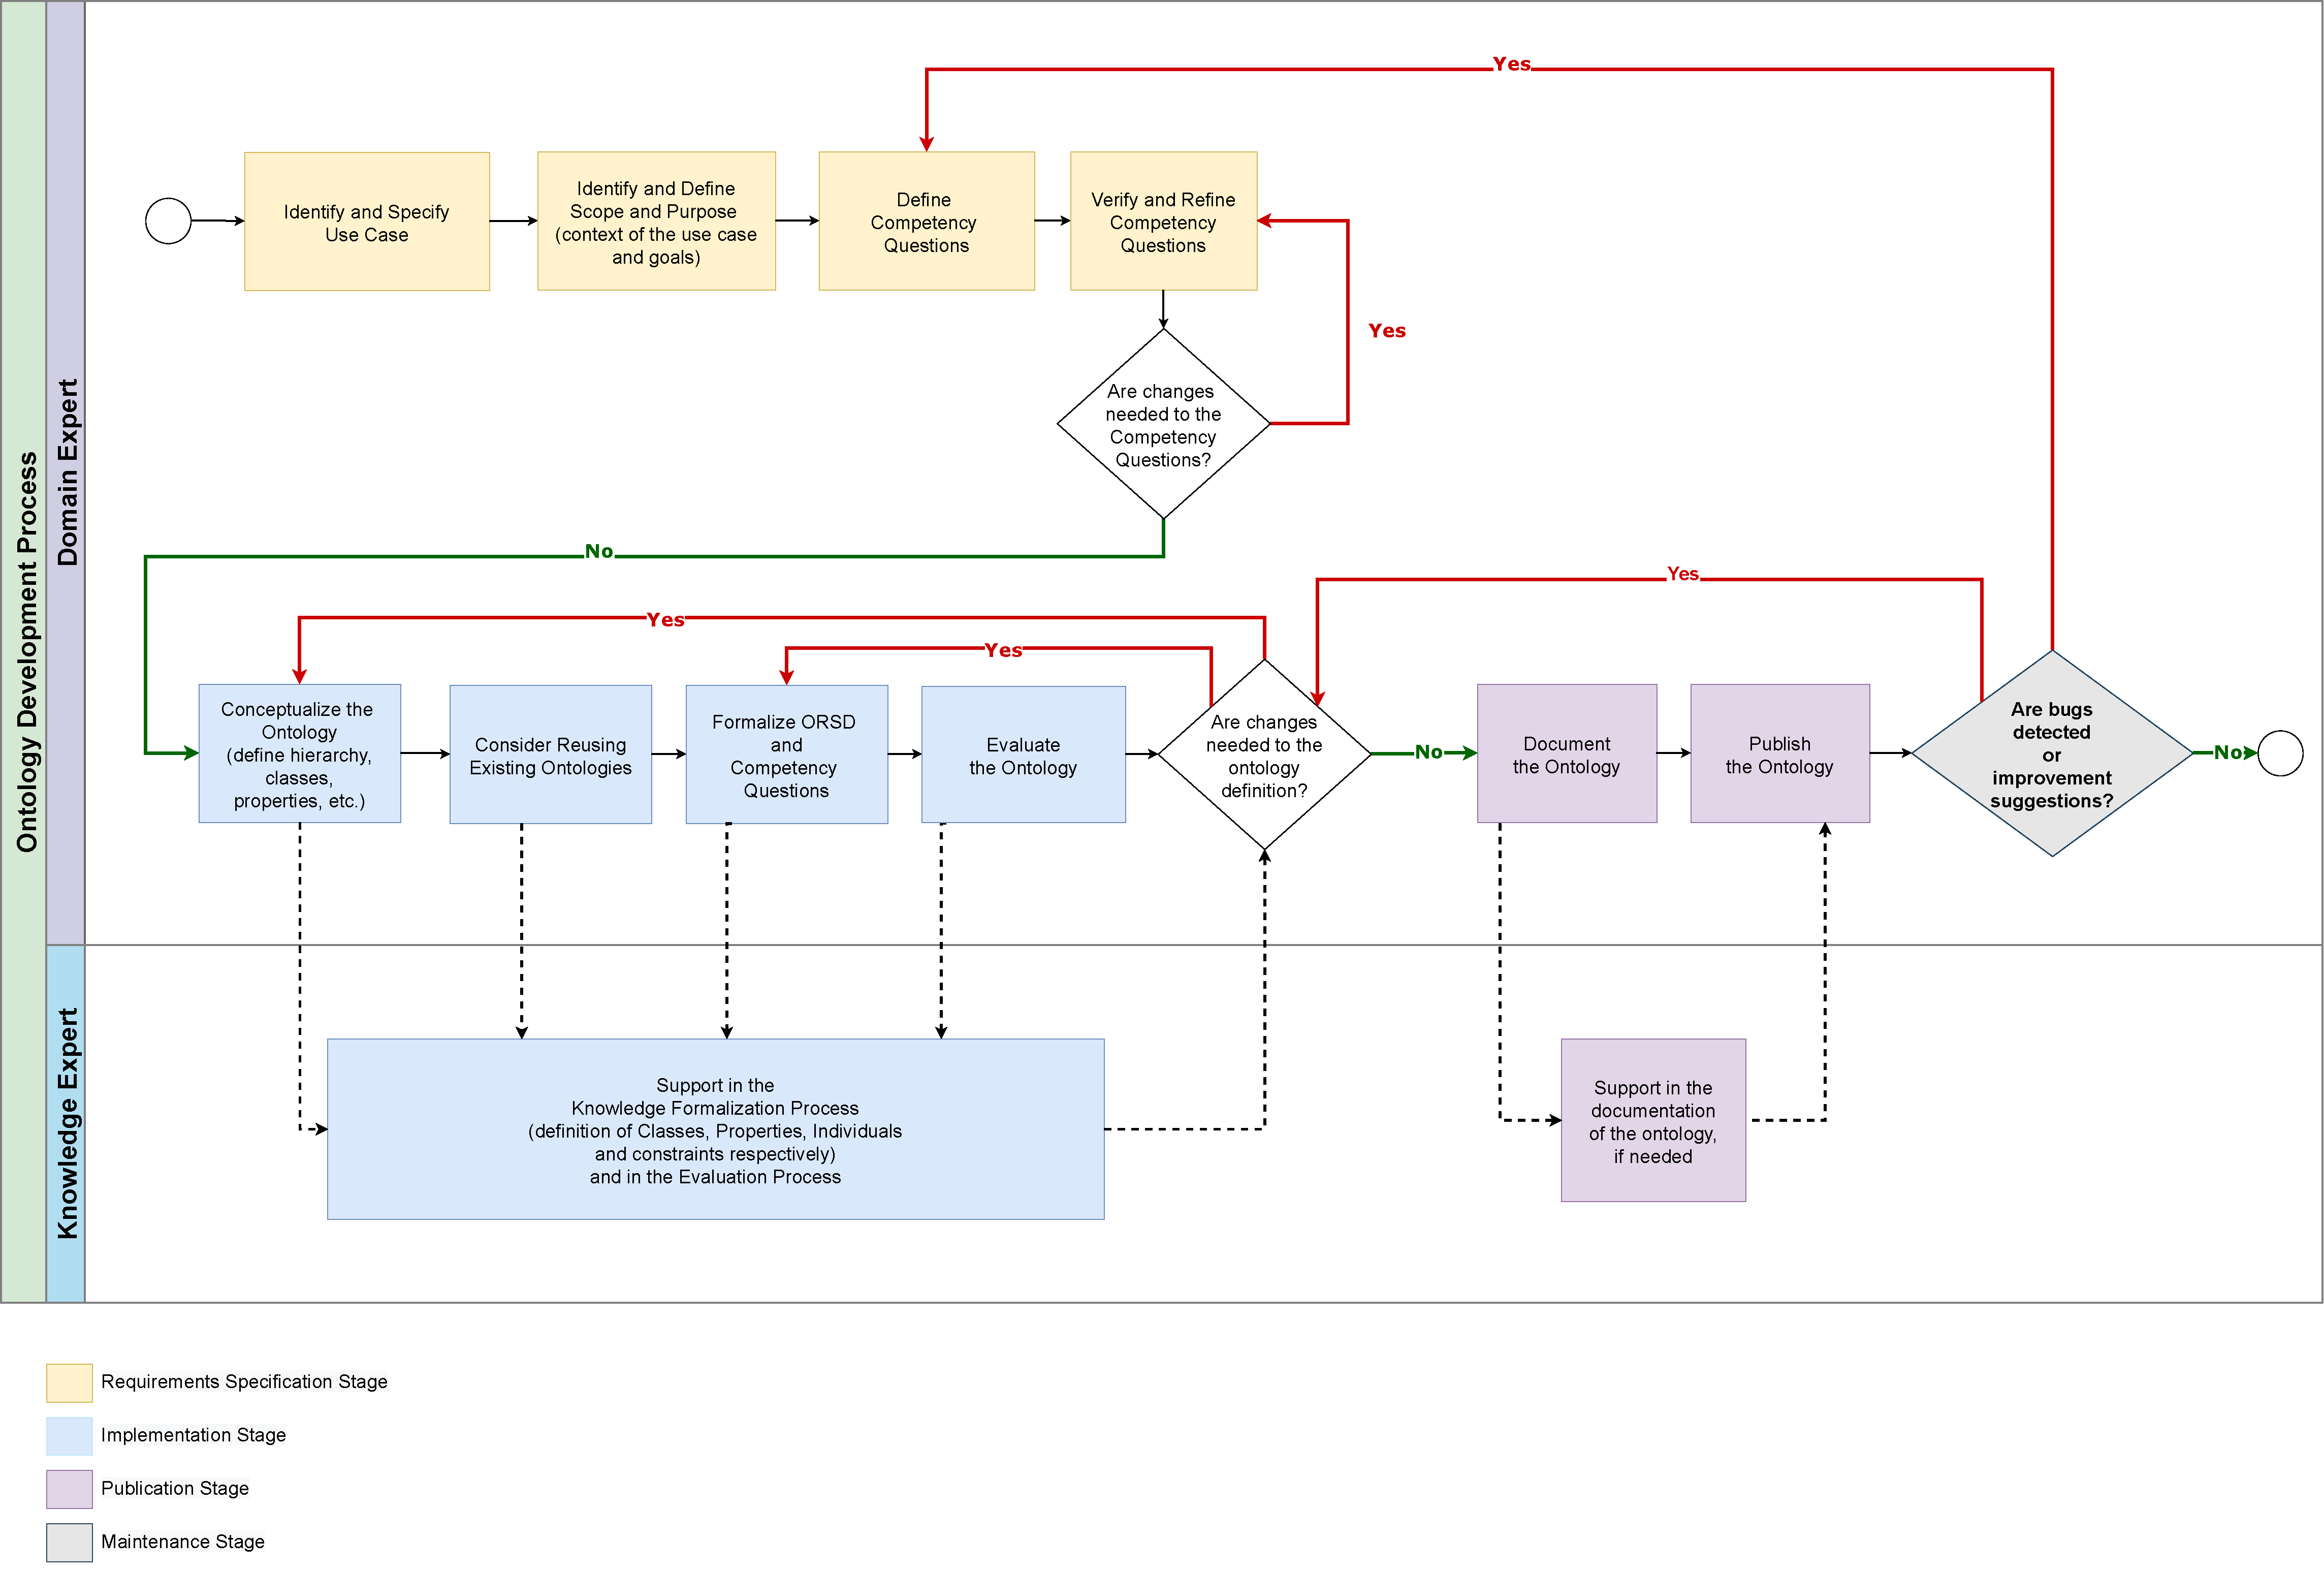
\includegraphics[width=1\textwidth]{images/adaptedworkflow.pdf}
      \caption{Ontology Development Workflow, our own definition based on the LOT methodology \cite{Poveda22}}
    \label{fig:workflowsuggestion}
\end{sidewaysfigure}

\subsection{Additional Resources} \label{sec:additionalresources}
For more detailed information and examples about the initial ontology development steps, we recommend reading the \textit{Ontology 101} report. Moreover, it is relevant to consider the resources in the \textit{NeOn Book} \cite{Perez08}, which we present here to help to go more in-depth on a specific topic.

\begin{table}[H]
	\centering
	\rowcolors{1}{unitednationsblue!20}{}
	\begin{tabular}{l}
		\hline
		\rowcolor{oceanboatblue!20} 
		\textbf{Additional Informational Resources} \\
		\hline
		\href{https://protege.stanford.edu/publications/ontology_development/ontology101.pdf}{Ontology101 (How to start and examples)} \\
		\href{http://neon-project.org/nw/book-chapters/Chapter-05.pdf}{Ontology Requirements Specification}\\
		\href{http://neon-project.org/nw/book-chapters/Chapter-09.pdf}{Reusing general ontologies}\\
		\href{http://neon-project.org/nw/book-chapters/Chapter-10.pdf}{Reusing domain ontologies}\\
		\href{http://neon-project.org/nw/book-chapters/Chapter-11.pdf}{How to reuse ontology statements}\\
		\href{http://neon-project.org/nw/book-chapters/Chapter-12.pdf}{How to model using Ontology Design Patterns (\ac{ODPs})}\\
        \href{http://neon-project.org/nw/book-chapters/Chapter-14.pdf}{How to approach ontology evaluation}\\
        \href{http://neon-project.org/nw/book-chapters/Chapter-15.pdf}{How to approach ontology modularization}\\
        \href{http://neon-project.org/nw/book-chapters/Chapter-16.pdf}{How to approach ontology evolution}\\
        \href{http://neon-project.org/nw/book-chapters/Chapter-17.pdf}{How to align ontologies in a network of ontologies}\\
        \href{http://neon-project.org/nw/NeOn_Book.html}{Complete NeOn Book with examples of large ontologies use cases}\\
		\hline
	\end{tabular}
    \caption{Additional resources to consider when developing ontologies} 
	\label{tab:additionalresources}
\end{table}

Moreover, the LOT methodology provides helpful links in the \textbf{"Recommended reads"} section associated with each activity (ontology requirements specification, ontology implementation, ontology publication, and ontology maintenance) in \url{https://lot.linkeddata.es}.

\newpage
\section{Best Practices} \label{sec:bestpractices}

Here we enumerate the most common best practices to consider when building an ontology, based on the existing literature. \singlespacing

\begin{enumerate}
\item \textbf{Decide} the following:
    \begin{itemize}
        \item Do we need to add a new class? 
        \item Do we need to model this entity as a new class or a property value?
        \item Do we need to model a disjointness of classes? 
        \item Is our class hierarchy correct and reflecting our use case? \label{item:classhierarchy}
    \end{itemize}
    \item \textbf{Reuse ontologies} instead of building a new one entirely from scratch, reusing them results in time-saving and improvement in the interoperability of the new ontology with the existing ones. \label{item:reuse}
    \item \textbf{Consider using Ontology Design Patterns (\ac{ODPs})}, as they are small ontology building blocks. \label{item:useodp}
    \item \textbf{Consider the quality requirements the new ontology should meet}. For instance, the ontology should be concise, modular, adaptable to different granularities and perspectives, and highly reusable while focusing on modelling only one essential notion of a domain.
    \item \textbf{Focus on upper (top-level) ontologies} to support consistent ontology development across domains. \label{item:toplevel}
    \item \textbf{Adopt the \textit{Top-Down} approach}, in which one defines first the most general concepts in the domain as a data schema and then applies gradual refinement of terms. \label{item:topdown}
    \item \textbf{Adopt a modular approach}, especially when designing large ontologies. It helps to facilitate reuse, extensibility and maintainability of the ontology.
    \item \textbf{Specify disjointness of classes} to help in the validation process. Two classes are disjoint if they cannot have any instances in common.
    \item \textbf{Consistency in classes name}, choose to use singular or plural when naming classes and keep it throughout the whole ontology creation.
    \item \textbf{Avoid class cycles}, pay attention when creating a class B as a subclass of A and then defining B as a superclass of A.
    \item \textbf{Follow name conventions}
    \begin{itemize}
        \item Capitalize the first letter of the class name and use lower case for naming the properties, e.g. \textit{Machine}, and \textit{produces}.
        \item When a concept name has more than one word, consider the following: either capitalize the first letter of each new word, or use an underscore, e.g. \textit{MachineComponent}, and \textit{Machine\_Component}.
        \item Avoid abbreviations in naming classes, properties, and individuals, e.g. \textit{Machine} instead of \textit{Mach}.
        \item Use prefixes in the property names, e.g. \textit{hasPart}.
    \end{itemize}
\end{enumerate} \singlespacing

\begin{beware} [Remark]
Regarding the class hierarchy in the ontology, presented in point \textbf{\ref{item:classhierarchy}}, recall that as \textit{ontology} is a philosophical concept, it is fundamental to understand the intentional structure of the things one describes through an ontology as they help appropriately classify concepts. The intentional structures one should consider are: \textit{1)} the intention of identifying things \textit{(continuants)} and \textit{2)} the intention of explaining things \textit{(occurrents)} \cite{Neuenschwander22}.\singlespacing
\end{beware}

\begin{beware}[Remark]
Additionally, there are other specific modelling principles to consider when focusing on ontologies in the production and manufacturing domain, such as those presented in \cite{BedenCao21,Psarommatis22,Zhou21}. Also, there are more general best practices in \cite{Rudnicki16} to help avoid the creation of heterogeneous and non-reusable ontologies. 
\end{beware}


\subsection*{How to use Ontology Design Patterns?}

Regarding the best practice in point \textbf{\ref{item:useodp}}, \ac{ODPs} are a reusable solution for recurrent modelling problems \cite{Jaskolka15,Shimizu19} and help to tackle the ontological commitment problem \footnote{Ontological commitment focuses on identifying the entities to be modelled into an ontology \cite{RodriguezDoncel15}}. They should be flexible, easily understandable and generic to support similar problems. \singlespacing

To better understand the concept of \ac{ODPs}, we present a small use case in Fig. \textbf{ \ref{fig:odpexample}}, based on the work presented in \cite{Presutti08}, in which we show how to use the \textit{``part of"} pattern. This pattern corresponds to the Content \ac{ODPs}. \singlespacing

In the scenario we describe here, \textbf{Filter}, \textbf{Valve}, \textbf{Motor} and \textbf{Port} are all components of the \textbf{Engine Stretch Blow Moulding}, which is expressed by the relation \textit{owl:unionOf}\footnote{\url{https://www.w3.org/TR/owl-ref/\#unionOf-def}} combined with the relation \textit{partof:hasPart}. At the same time, \textbf{Engine Stretch Blow Moulding} is part of \textbf{Machine Stretch Moulding}, we know that by the relation \textit{partof:hasPart} between those two entities. Therefore, by transitivity property of the relationships among entities, we see that it can be inferred that \textbf{Filter},\textbf{ Valve}, \textbf{Motor} and \textbf{Port} are also part of \textbf{Machine Stretch Moulding} (blue dotted lines).\singlespacing

    \begin{figure}[H]
        \centering
          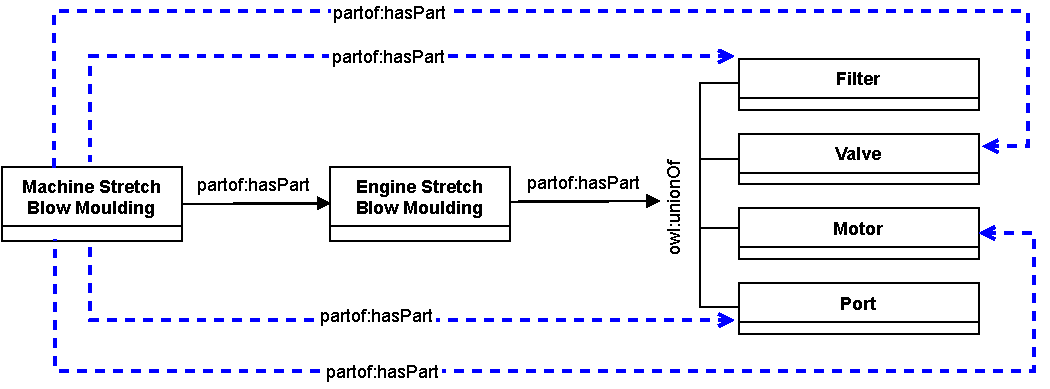
\includegraphics[width=1\textwidth]{images/ODPexample.pdf}
          \caption{An example of the Content \ac{ODPs} ``part of"}
        \label{fig:odpexample}
    \end{figure}
    
\begin{beware} [Note]
In Section \textbf{\ref{sec:additionalresources}} we provide a link to the document \textit{How to model using ODPs}. \singlespacing
\end{beware}

\newpage
%%%%%%%%%%%%%%%%%%%%%%%%%%%%%%%%%%%%%%%%%%%%%%%%%%%
%% Tools
%%%%%%%%%%%%%%%%%%%%%%%%%%%%%%%%%%%%%%%%%%%%%%%%%%%
\section{Tools}
\label{sec:tools}
There are several tools to be considered when developing ontologies. Here we recommend the required tools to create an ontology. In Fig. \textbf{\ref{fig:toolstages}} we name these tools corresponding to each stage of the ontology development. \singlespacing

    \begin{figure}[H]
        \centering
          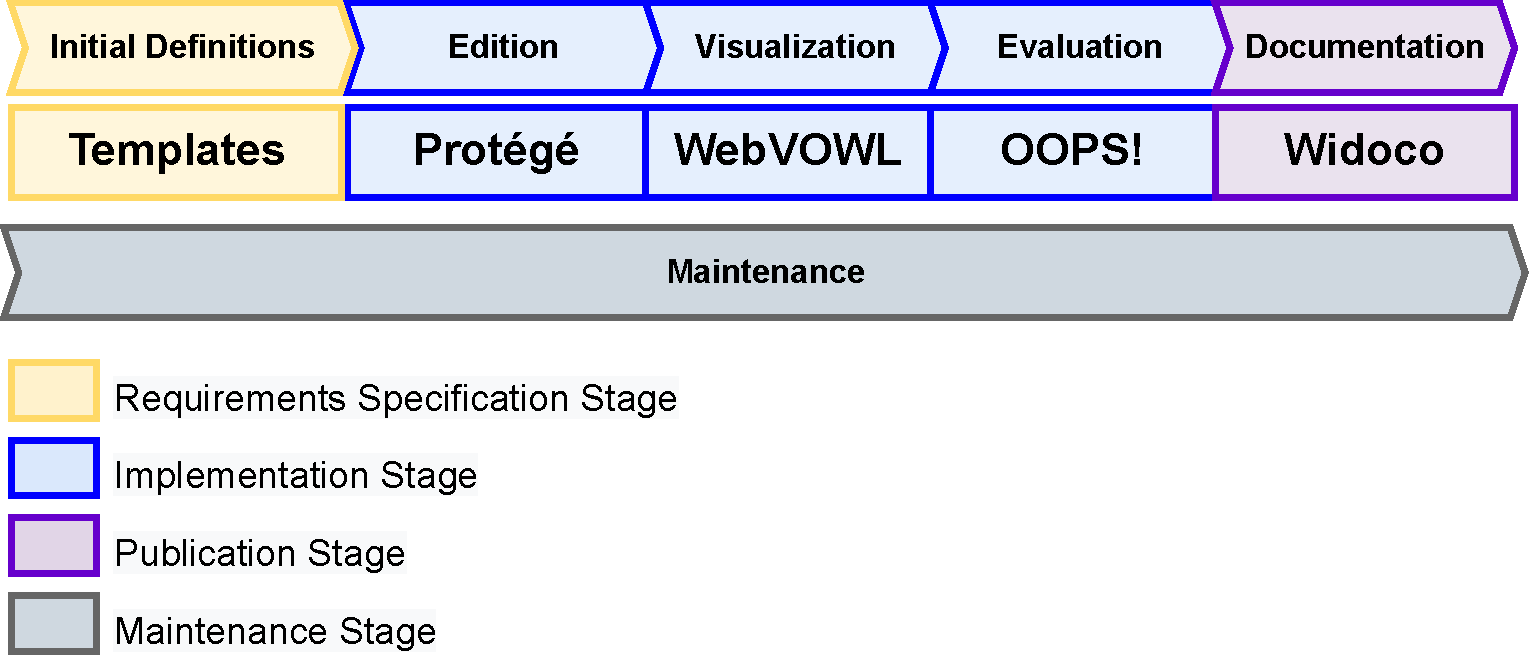
\includegraphics[width=1\textwidth]{images/Tools-Stages.pdf}
          \caption{Tools needed at each stage of the ontology development process}
        \label{fig:toolstages}
    \end{figure}
    
\begin{beware}[Remark]
In Section \textbf{\ref{subsec:additionaltools}} we present tools that one should consider when developing ontologies. They are not mandatory for starting the modelling process. However, knowing and understanding them brings additional benefits.
\end{beware}

\subsection{Tool Tutorials and Additional Resources}
In Table \textbf{\ref{tab:toolresources}} we provide the necessary links to tutorials and additional resources to reference when using these tools.
    
\begin{table}[H]
	\centering
	\rowcolors{1}{unitednationsblue!20}{}
	\begin{tabular}{l}
		\hline
		\rowcolor{oceanboatblue!20} 
		\textbf{Tool Resources and Tutorials} \\
		\hline
		\href{http://protegeproject.github.io/protege/getting-started/}{Getting started with Protégé} \\
		\href{https://buildmedia.readthedocs.org/media/pdf/go-protege-tutorial/latest/go-protege-tutorial.pdf}{Protégé Tutorial} \\
		\href{https://protegewiki.stanford.edu/wiki/Importing_Ontologies_in_P41}{How to import ontologies in Protégé?} \\
		\href{https://stackoverflow.com/questions/44205661/how-to-import-specific-classes-and-object-properties-from-an-ontology-in-protegeQ}{How to import only some classes and properties in Protégé?} \\
		\href{http://vowl.visualdataweb.org/v2/}{Documentation and Notations of VOWL, WebVOWL} \\
		\href{https://oops.linkeddata.es/OOPSUserGuidev1.pdf}{OOPS! User Guide} \\
		\href{https://dgarijo.github.io/Widoco/doc/tutorial/}{Widoco Tutorial} \\
		\hline
	\end{tabular}
    \caption{Tool resources and tutorials} 
	\label{tab:toolresources}
\end{table}

\newpage
\subsection{Where to Find the Recommended Tools}
Additionally, in Table \textbf{\ref{tab:findingtools}}, we provide the links for finding and downloading the tools, if necessary.

\begin{table}[H]
	\centering
	\rowcolors{1}{unitednationsblue!20}{}
	\begin{tabular}{l}
		\hline
		\rowcolor{oceanboatblue!20} 
		\textbf{Where to find the tools} \\
		\hline
		\href{https://drive.google.com/drive/folders/1xwtJYaNQIGd1TWdWayciCiH5wcpnSDxw?usp=sharing}{Templates} \\
		\href{https://protege.stanford.edu/products.php#desktop-protege}{Protégé Desktop} \\
		\href{https://webprotege.stanford.edu}{Protégé Web} \\
		\href{https://service.tib.eu/webvowl/}{WebVOWL} \\
		\href{https://oops.linkeddata.es}{OOPS!} \\
		\href{https://github.com/dgarijo/WIDOCO/releases/tag/v1.4.17}{Widoco} \\
		\hline
	\end{tabular}
    \caption{Finding the tools} 
	\label{tab:findingtools}
\end{table}

\begin{beware}[Remark]
Regarding \textit{Protégé} as an ontology creation and editing tool, we recommend using the desktop version, as one can extend it with plugins. There is also a web version which is a simplified version of the tool. \singlespacing
\end{beware}

\subsection{Further Tools to Advance the Ontology Development Process} \label{subsec:additionaltools}
In this section, we present some additional tools, which we recommend to the reader for enhancing their knowledge regarding the ontology development process. Such tools are the underlying standard languages for ontologies construction, ontology querying languages tools, versioning control tools, and languages for modelling constraints to validate the quality of the resulting ontology. \singlespacing

In Table \textbf{\ref{tab:additionaltoolresources}} we list these tools. The content in the first column is a clickable link to the tools documentation.

\begin{table}[H]
	\centering
	\rowcolors{1}{unitednationsblue!20}{}
	\begin{tabular}{L{.4\textwidth} L{.6\textwidth}}
		\hline
		\rowcolor{oceanboatblue!20} 
		\textbf{Advanced Tools} & \textbf{Description}   \\
		\hline
		\href{https://www.w3.org/TR/rdf11-concepts/}{Resource Description Framework (RDF)} & A framework for representing information in the Web, which serve as a base for all RDF-based languages \\
		\href{https://www.w3.org/TR/rdf-schema/}{RDF Schema (RDFS)} & Data-modelling vocabulary for RDF data \\
		\href{https://www.w3.org/TR/owl-overview/}{Web Ontology Language (OWL 2)} & An ontology language used to formally define the meaning of concepts \\
		\href{https://www.w3.org/TR/shacl/}{Shapes Constraint Language (SHACL)} & A data validation language to validate RDF graphs against user-defined conditions \\
		\href{http://shex.io/shex-semantics/}{Shape Expressions Language (ShEx)} & A data validation and generation language to describe RDF graphs and nodes structures\\
		\href{https://www.w3.org/TR/sparql11-query/}{SPARQL Query Language} & A graph querying language. The query results can be expressed as sets or RDF graphs \\
		\href{https://about.gitlab.com}{GitLab} & Version control tool. It is an open source code repository and collaborative development tool\\
		\href{https://github.com}{GitHub} & Version control tool. It is a code repository and collaborative development tool \\
		\hline
	\end{tabular}
    \caption{Advanced tools - Documentation} 
	\label{tab:additionaltoolresources}
\end{table}

\newpage
To complement the information and help the reader, we offer a starting point by providing links in Table \textbf{\ref{tab:additionaltooltutorials}} to some relevant tutorials introducing these more advanced tools.

\begin{table}[H]
	\centering
	\rowcolors{1}{unitednationsblue!20}{}
	\begin{tabular}{l}
		\hline
		\rowcolor{oceanboatblue!20} 
		\textbf{Advanced Tools - Tutorials} \\
		\hline
		\href{http://www.linkeddatatools.com/introducing-rdf-part-2}{Introducing RDF} \\
		\href{https://cgi.di.uoa.gr/~pms547/lectures/introduction-to-rdf-schema-revised-1spp.pdf}{Introduction to RDFS} \\
		\href{https://protege.stanford.edu/conference/2006/submissions/slides/OWLTutorial\_Part1.pdf}{OWL Tutorial} \\
		\href{https://en.wikibooks.org/wiki/SPARQL}{SPARQL Book} \\
		\href{http://www.linkeddatatools.com/querying-semantic-data}{Querying Semantic Data} \\
		\href{https://data.europa.eu/sites/default/files/d2.1.2\_training\_module\_1.3\_introduction\_to\_rdf\_sparql\_en\_edp.pdf}{Introduction to RDF and SPARQL} \\
		\href{http://www.linkeddatatools.com/introducing-rdfs-owl}{Introducing RDFS and OWL} \\
		\href{https://www.ida.liu.se/~robke04/SHACLTutorial/Introduction\%20to\%20SHACL.pdf}{Introduction to SHACL} \\
		\href{http://www.weso.es/RDFValidation\_ESWC16/slides/ShExByExample.pdf}{ShEx by Example} \\
		\href{https://www.youtube.com/watch?v=RGOj5yH7evk}{Videotutorial - Git and GitHub for Beginners} \\
		\href{https://docs.github.com/en/get-started/quickstart}{GitHub Quickstart} \\
		\href{https://opensource.com/article/18/1/step-step-guide-git}{A step-by-step guide to Git} \\
		\href{https://docs.github.com/en/desktop/installing-and-configuring-github-desktop/overview/getting-started-with-github-desktop}{Getting started with GitHub Desktop} \\
		\href{https://opensource.com/article/18/1/step-step-guide-git}{Learn GitLab with tutorials} \\
		\hline
	\end{tabular}
    \caption{Advanced Tools - Tutorials} 
	\label{tab:additionaltooltutorials}
\end{table}

In Table \textbf{\ref{tab:moreadditionaltools}} we list a broader set of tools to support the ontology development process. We consider these tools relevant because they provide visual support to create queries or to generate ontologies from diagrams. They can used together with the main tools we introduced at the beginning of this section.


\begin{table}[H]
	\centering
	\rowcolors{1}{unitednationsblue!20}{}
	\begin{tabular}{L{.25\textwidth} L{.75\textwidth}}
		\hline
		\rowcolor{oceanboatblue!20} 
		\textbf{Additional Tools} & \textbf{Description} \\
		\hline
		\href{https://sparql-playground.sib.swiss}{SPARQL Playground} & A tool for learning and testing SPARQL\\
		\href{http://sparqlblocks.org}{SparqlBlocks} & A library to visually build SPARQL queries using blocks \\
		\href{https://github.com/sparna-git/Sparnatural}{Sparnatural} & A visual tool to build SPARQL queries \\
		\href{https://chowlk.linkeddata.es}{Chowlk Converter} & A tool to generate ontologies in OWL from a conceptualization diagram \\
		\href{https://github.com/Semantic-Society/Neologism}{Neologism 2.0} & A visual tool for quick vocabulary creation \\
		\href{http://semantics.istc.cnr.it/frodo}{FrODO} & A tool for automatically drafting ontologies from competency questions \\
		\href{https://comodide.com}{CoModIDE} & A plugin for Protégé for graphical composition of ontologies\\
		\href{https://gitlab.ifi.uzh.ch/DDIS-Public/chimp-protege-plugin}{ChImp} & A plugin for Protégé to verify changes in the ontologies and visually analyse their impact\\
		\hline
	\end{tabular}
    \caption{Additional Tools} 
	\label{tab:moreadditionaltools}
\end{table}

\newpage
%%%%%%%%%%%%%%%%%%%%%%%%%%%%%%%%%%%%%%%%%%%%%%%%%%%
%% Templates
%%%%%%%%%%%%%%%%%%%%%%%%%%%%%%%%%%%%%%%%%%%%%%%%%%%
\section{Templates} \label{sec:templates}

To download the templates, please refer to the following link to a Google Drive Folder: \href{https://drive.google.com/drive/folders/1xwtJYaNQIGd1TWdWayciCiH5wcpnSDxw?usp=sharing}{GuidelineForCreationSemanticModelsIoP}, in which the following templates are available: \ac{ORSD}, Competency Questions Definition, Class Definition, Property Definition, and Individuals Definition. \singlespacing

In the following, we briefly describe what each template is. Moreover, inside each available template, we provide additional links to resources to use when needed. These supplementary resources can help to clarify concepts and to observe examples. 

\subsection{Ontology Requirements Specification}
One can use the template \href{https://docs.google.com/document/d/1mkHccxvvGbj3omXubZ_EbM_l7m8LfalJ/edit}{\textit{Template\_OntologyRequirementsSpecification}} to define the purpose and scope of the ontology. It also helps to determine the intended uses and end-users of the ontology. It is complemented with the \href{https://docs.google.com/spreadsheets/d/1UwT7DnW3pIkDKmfn1jgONsp2BbiQZ4mJeeg0lOBV0DQ/edit#gid=0}{\textit{Template\_CompetencyQuestions\_Definition}} to determine the ontology requirements.

\subsection{Competency Questions Definition}
The \href{https://docs.google.com/spreadsheets/d/1UwT7DnW3pIkDKmfn1jgONsp2BbiQZ4mJeeg0lOBV0DQ/edit#gid=0}{\textit{Template\_CompetencyQuestions\_Definition}} helps to define the questions that the ontology should be able to answer once the modelling process is complete. They are also used to identify the important terms in the ontology. Those important terms then can be defined by using the \href{https://docs.google.com/spreadsheets/d/16g3pAnE-fzbQydI0m5zkswAc83r881oBgKarQaCkGa0/edit#gid=0}{\textit{Template\_Class\_Definition}}, \href{https://docs.google.com/spreadsheets/d/1pmVIaY3WwofKMBwXdqbiCgXH5DL4rNx-ZhKlHUdZoRo/edit#gid=0}{\textit{Template\_Property\_Definition}} , and \href{https://docs.google.com/spreadsheets/d/11_twMjg6mwAQoefg4pRDqZCcsNCKwbrflg0NIkcyF1I/edit#gid=0}{\textit{Template\_Individuals\_Definition}} templates. \singlespacing

Additionally, Competency Questions are commonly used to evaluate the newly created ontology, as one has to ensure that the ontology contains enough information to answer these questions.

\subsection{Class Definition}
The \href{https://docs.google.com/spreadsheets/d/16g3pAnE-fzbQydI0m5zkswAc83r881oBgKarQaCkGa0/edit#gid=0}{\textit{Template\_Class\_Definition}} helps to identify and define the classes in the ontologies. Classes are collections of objects, e.g. \textit{Machine, Product} etc.

\subsection{Property Definition}

The \href{https://docs.google.com/spreadsheets/d/1pmVIaY3WwofKMBwXdqbiCgXH5DL4rNx-ZhKlHUdZoRo/edit#gid=0}{\textit{Template\_Property\_Definition}} helps to identify and define the properties in the ontologies. Properties, also called slots, are the attributes describing one or more classes, e.g. \textit{hasVolume, hasResponsible, hasPart} etc.

\subsection{Individuals Definition}
The \href{https://docs.google.com/spreadsheets/d/11_twMjg6mwAQoefg4pRDqZCcsNCKwbrflg0NIkcyF1I/edit#gid=0}{\textit{Template\_Individuals\_Definition}} helps to identify and define the individuals in the ontologies. Individuals are instances of classes having an associated value, e.g. \textit{Resistor\_01} etc.

\newpage
%%%%%%%%%%%%%%%%%%%%%%%%%%%%%%%%%%%%%%%%%%%%%%%%%%%
%% Architectural Suggestions
%%%%%%%%%%%%%%%%%%%%%%%%%%%%%%%%%%%%%%%%%%%%%%%%%%%

\section{How to build ontologies for the IoP?} \label{sec:architecturalsuggestions}

To start building the ontology by using the methodology presented in Chapter \textbf{\ref{sec:methodologies}} and the tools indicated in Chapter \textbf{\ref{sec:tools}}, you need to consider the best practices we mentioned in Chapter \textbf{\ref{sec:bestpractices}}. \singlespacing

Regarding the best practice in point \textbf{\ref{item:reuse}}, here we present a suggestion to build your new ontology. There are two possibilities: \singlespacing

\begin{itemize}
    \item \textbf{New ontology uses support ontologies:} we recommended this style when modelling domain-specific ontologies, including non-technical concepts from the manufacturing and production domain, such as organizational and administrative knowledge. \label{item:supportontologiesused}
    \item \textbf{New ontology does not need to use support ontologies:} we recommend this style when modelling only domain-specific knowledge. \label{item:supportontologiesnotused}
\end{itemize} \singlespacing

In Fig. \textbf{\ref{fig:ontologyarchitecture}} we show what the new ontology would look like by reusing existing ontologies. It is a composition of the upper (top-level) ontology, domain-specific ontologies, and support ontologies.

\begin{figure}[H]
    \begin{subfigure}[t]{0.45\textwidth}
        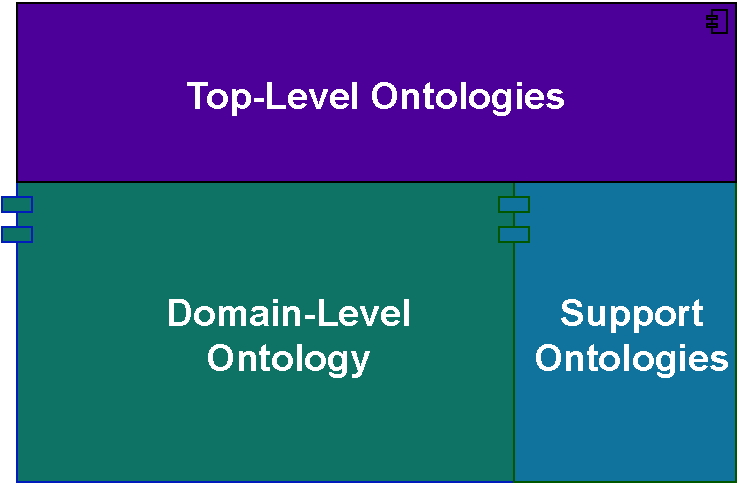
\includegraphics[width=\textwidth,]{images/abstractarchitecture.pdf}
        \caption{Conceptual Ontology Architecture}
        \label{fig:abstractarchitecture}
    \end{subfigure}
    \hfill
    \begin{subfigure}[t]{0.45\textwidth}
        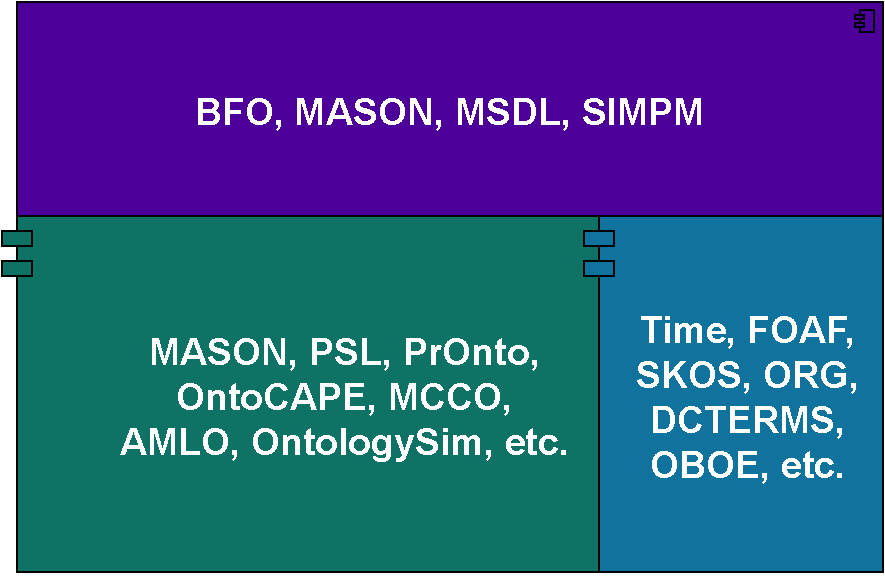
\includegraphics[width=\textwidth]{images/suggestedarchitecture.pdf}
        \caption{Suggested Ontology Architecture}
        \label{fig:suggestedarchitecture}
    \end{subfigure}
    \caption{Architecture for the Ontology Development in IoP by using General Ontologies}
    \label{fig:ontologyarchitecture}
\end{figure}

In Fig. \textbf{\ref{fig:ontologyarchitecture_withoutgeneralontologies}} we show how the new ontology would look by reusing existing ontologies but without using support ontologies because the model only covers domain-specific concepts. Then, it is a composition of the upper (top-level) ontology and domain-specific ontology or ontologies.

\begin{figure}[H]
    \begin{subfigure}[t]{0.45\textwidth}
        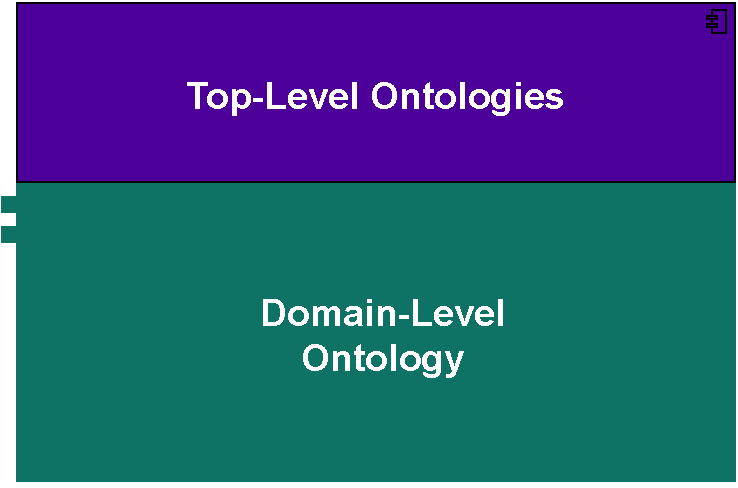
\includegraphics[width=\textwidth,]{images/abstractarchitecture2_guideline.pdf}
        \caption{Conceptual Ontology Architecture}
        \label{fig:abstractarchitecture2guideline}
    \end{subfigure}
    \hfill
    \begin{subfigure}[t]{0.45\textwidth}
        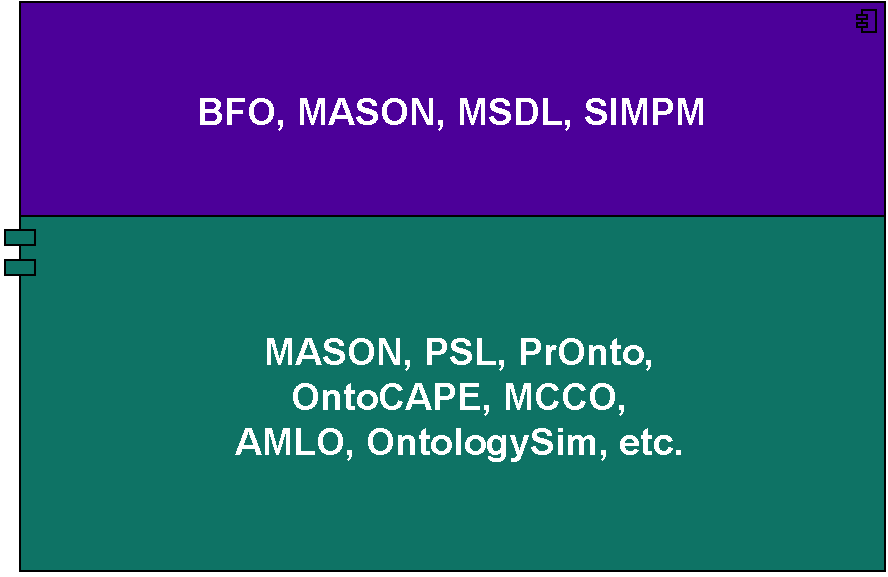
\includegraphics[width=\textwidth]{images/suggestedarch2_guidelines.pdf}
        \caption{Suggested Ontology Architecture}
        \label{fig:suggestedarch2_guidelines}
    \end{subfigure}
    \caption{Architecture for the Ontology Development in IoP without using General Ontologies}
    \label{fig:ontologyarchitecture_withoutgeneralontologies}
\end{figure}


%%%%%%%%%%%%%%%%%%%%%%%%%%%%%%%%%%%%%%%%%%%%%%%%%%%
%% Upper Ontologies 
%%%%%%%%%%%%%%%%%%%%%%%%%%%%%%%%%%%%%%%%%%%%%%%%%%%
\subsection{Upper (Top-Level) Ontologies}
\label{sec:upperontologies}

As we explained in Section \textbf{\ref{sec:classificationontologies}}, Upper or Top-Level Ontologies are generic and it is helpful to use them to start building a new ontology on top of them, as indicated in points \textbf{\ref{item:toplevel}} and \textbf{\ref{item:topdown}}. Therefore, in Table \textbf{\ref{tab:upperontologies}} we present a list of some important ontologies in this category. Each resource name is a link to access them.

\begin{table}[H]
	\centering
	\rowcolors{1}{unitednationsblue!20}{}
	\begin{tabular}{ll}
		\hline
		\rowcolor{oceanboatblue!20} 
		\textbf{Resource} & \textbf{Features}\\
		\hline
\href{https://www.avt.rwth-aachen.de/cms/AVT/Forschung/Sonstiges/Software/~ipts/OntoCape/?lidx=1}{OntoCape} & Process engineering  \\

\href{https://github.com/bfo-ontology/BFO/wiki}{BFO} & Information retrieval, analysis and integration in various domains \\

\href{https://www.onto-med.de/ontologies/gfo}{GFO} & Categories such as objects, processes, time and space, relations,roles, etc.  \\

\href{https://sourceforge.net/projects/mason-onto/}{MASON} & Automatic cost estimation and manufacturing simulation \\

SIMPM & Model constraints of manufacturing process planning: variety, time, and aggregation\\

MSDL & Represents conventional manufacturing processes \\

\href{http://www.hozo.jp/onto_library/upperOnto.htm}{YAMATO} & Quality and quantity, Objects, Processes and Events, etc. \\

\href{http://ontolog.cim3.net/wiki/COSMO.html}{COSMO} & Broad semantic interoperability \\

\href{https://www.semanticarts.com/gist/}{gist} & Maximum coverage of typical business ontology concepts \\

\hline
\end{tabular}
\caption{Upper and Middle Ontologies} \label{tab:upperontologies}
\end{table}

%%%%%%%%%%%%%%%%%%%%%%%%%%%%%%%%%%%%%%%%%%%%%%%%%%%
%% Support Ontologies - Ontologies Supporting integration with IoP
%%%%%%%%%%%%%%%%%%%%%%%%%%%%%%%%%%%%%%%%%%%%%%%%%%%
\subsection{Support Ontologies: Ontologies Supporting integration with IoP}
\label{sec:supportontologies}

Here we present some valuable ontologies and standard vocabularies for modelling cross-domain concepts such as organization structure, time and measurement concepts. \singlespacing

In Table \textbf{\ref{tab:currentsupportontologies}}, the column \textit{"Resource"} provides the name and an URL to access the documentation of the ontology or vocabulary. In column \textit{"Features"} we briefly describe the scope of the resource.

\begin{table}[H]
	\centering
	\rowcolors{1}{unitednationsblue!20}{}
	\begin{tabular}{ll}
		\hline
		\rowcolor{oceanboatblue!20} 
		\textbf{Resource} & \textbf{Features} \\
		\hline
\href{https://www.w3.org/TR/vocab-org/}{ORG} & Describe organizational structures \\ 
\href{https://www.w3.org/TR/owl-time/}{Time} & Represent temporal concepts \\ 
\href{https://www.w3.org/TR/vcard-RDF/}{vCard} & Promote the use of vCard for the description of people and organisations  \\ 
\href{https://www.w3.org/2009/08/skos-reference/skos.html}{SKOS} & Promote sharing and linking knowledge organization systems \\ 
\href{http://xmlns.com/foaf/spec/}{FOAF} & Describe set of concepts and properties linking people and information\\ 
\href{https://www.qudt.org}{QUDT} & Represent various quantity and unit standards \\
\href{https://www.dublincore.org/specifications/dublin-core/dcmi-terms/}{DCMI-Terms} & Specifies metadata terms \\
\href{https://www.w3.org/TR/vocab-data-cube/}{RDFDataCube} & Publication of multi-dimensional data on the web \\ 
\href{https://www.w3.org/TR/qb4st/}{QB4ST} & Extension of RDF Data Cube ontology to describe Spatio-temporal data \\ 
\href{https://github.com/HajoRijgersberg/OM}{OM} & Helps to model concepts and relations important to scientific research \\
\href{https://nfdi4ing.pages.rwth-aachen.de/metadata4ing/metadata4ing/index.html#}{Metadata4Ing} & Helps to describe the generation of research data within a scientific activity \\
\href{https://www.w3.org/TR/vocab-dcat-2/}{DCAT} & It allows the description of data catalogs published on the Web \\
\href{https://www.w3.org/TR/prov-o/}{PROV-O} & It allows integrating domains provenance in the information \\
\href{https://www.w3.org/TR/void/}{VoID} & It helps in describing metadata about RDF datasets \\
\href{https://www.w3.org/TR/vocab-dqv/}{DQV} & It allows to express concepts related to data quality \\
\hline
\end{tabular}
\caption{Support Ontologies} 
\label{tab:currentsupportontologies}
\end{table}

\newpage
%%%%%%%%%%%%%%%%%%%%%%%%%%%%%%%%%%%%%%%%%%%%%%%%%%%
%% Domain Ontologies in IoP
%%%%%%%%%%%%%%%%%%%%%%%%%%%%%%%%%%%%%%%%%%%%%%%%%%%
\subsection{Domain Ontologies: Ontologies in IoP}
\label{sec:domainontologies}

There exist various domain-specific ontologies in the manufacturing and production domain. Some of these and other ontologies can be found by following the links we present in Section \textbf{\ref{sec:catalogues}}. \singlespacing

In the Appendix, in Section \textbf{\ref{sec:detaileddomainontologies}} we present the list of domain ontologies in the manufacturing and production domain by including the respective references in case you want to explore them more in-depth.

%%%%%%%%%%%%%%%%%%%%%%%%%%%%%%%%%%%%%%%%%%%%%%%%%%%
\subsection{Catalogue}
\label{sec:catalogues}

Here we present a catalogue of resources to localize some of the ontologies mentioned in the previous sections. Each resource name is a link to access them. We also added comments on how to use these resources.

\begin{table}[H]
	\centering
	\rowcolors{1}{unitednationsblue!20}{}
	\begin{tabular}{L{.35\textwidth} L{.65\textwidth}}
		\hline
		\rowcolor{oceanboatblue!20} 
		\textbf{Resource} & \textbf{Comments} \\
		\hline
		\href{https://terminology.nfdi4ing.de/ts4ing/index}{NFDI4Ing Terminology Service} & It has search option by terms and list of ontologies\\
		\href{https://lov.linkeddata.es/dataset/lov}{Linked Open Data} & One can filter by tag, for example, by tag ``industry" \\
        \href{https://ontohub.org/ontologies}{Ontohub} & It has different filters such as ontology type \\
        \href{https://www.vocoreg.com}{VoCol Service} & It has a search option by term and an search by ontology \\
        \href{https://bartoc.org/vocabularies}{Bartoc} & It has a search option and also a filtering system \\
        \href{https://data.ontocommons.linkeddata.es/index}{Ontocommons} & A list of ontologies in the manufacturing domain and other industries \\
        \href{https://github.com/search?q=ontology}{Ontologies in GitHub} & A search by keyword ``ontology" \\
        \href{http://ontologydesignpatterns.org/wiki/Ontology:Main}{ODP ontologies} & A catalogue of exemplary ontologies \\
		\hline
	\end{tabular}
    \caption{Ontologies and Vocabularies Catalogues} 
	\label{tab:catalogs}
\end{table}

  
%%%%%%%%%%%%%%%%%%%%%%%%%%%%%%%%%%%%%%%%%%%%%%%%%%%
%% Bibliography 
%%%%%%%%%%%%%%%%%%%%%%%%%%%%%%%%%%%%%%%%%%%%%%%%%%%
\MyBibliography

\newpage
\appendix
\section{Appendix}

\subsection{LOT Methodology Figures} \label{sec:lotfigure}

    \begin{figure}[H]
        \centering
          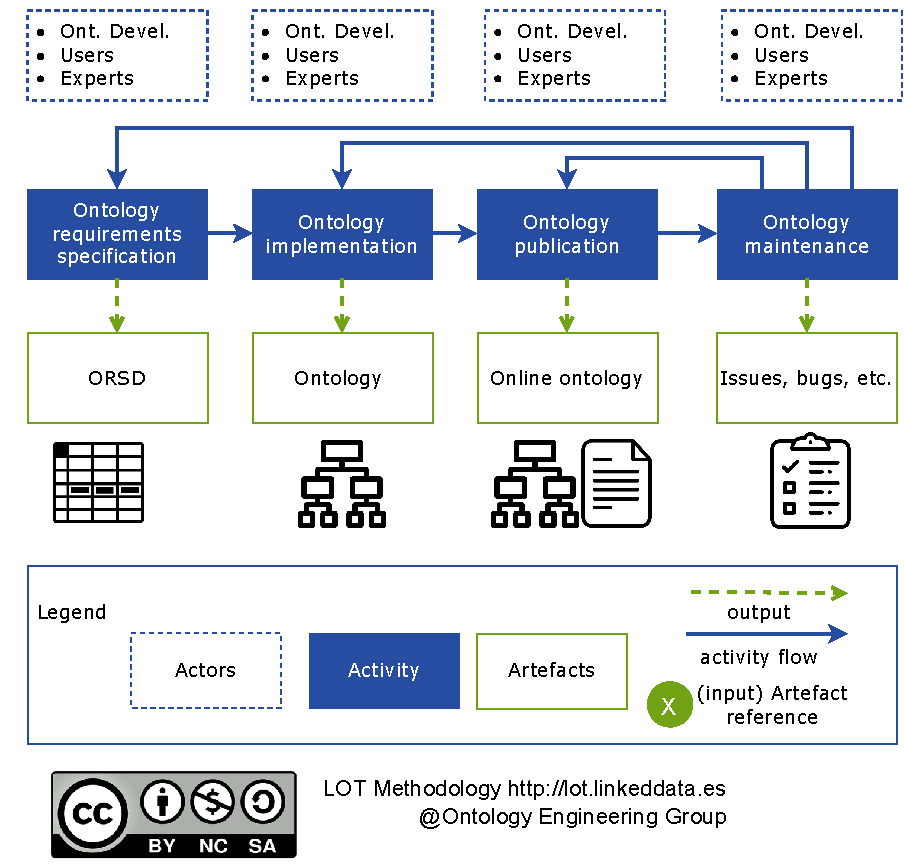
\includegraphics[width=\textwidth]{images/LOTFigure1.pdf}
          \caption{LOT Methodology Overview \\ Ontological Engineering Group (OEG). Licensed under a Creative Commons Attribution-NonCommercial-ShareAlike 4.0 International License}
    \label{fig:lotfigure1}
    \end{figure}
    
     \begin{figure}[H]
        \centering
          \includegraphics[width=1.1\textwidth]{images/LOTFigure2.pdf}
          \caption{LOT Methodology Detailed View \\ Ontological Engineering Group (OEG). Licensed under a Creative Commons Attribution-NonCommercial-ShareAlike 4.0 International License}
    \label{fig:lotfigure2}
    \end{figure}
    
       \begin{figure}[H]
        \centering
          \includegraphics[width=1.1\textwidth]{images/LOTFigure3.pdf}
          \caption{LOT Methodology - Stage: Ontology Requirements Specification \\ Ontological Engineering Group (OEG). Licensed under a Creative Commons Attribution-NonCommercial-ShareAlike 4.0 International License}
    \label{fig:lotfigure3}
    \end{figure}
    
    \begin{figure}[H]
        \centering
          \includegraphics[width=1.1\textwidth]{images/LOTFigure4.pdf}
          \caption{LOT Methodology - Stage: Ontology Implementation \\ Ontological Engineering Group (OEG). Licensed under a Creative Commons Attribution-NonCommercial-ShareAlike 4.0 International License}
    \label{fig:lotfigure4}
    \end{figure}
    
    \begin{figure}[H]
        \centering
          \includegraphics[width=1.1\textwidth]{images/LOTFigure5.pdf}
          \caption{LOT Methodology - Stage: Ontology Publication \\ Ontological Engineering Group (OEG). Licensed under a Creative Commons Attribution-NonCommercial-ShareAlike 4.0 International License}
    \label{fig:lotfigure5}
    \end{figure}
    
        \begin{figure}[H]
        \centering
          \includegraphics[width=\textwidth]{images/LOTFigure6.pdf}
          \caption{LOT Methodology - Stage: Ontology Maintenance \\ Ontological Engineering Group (OEG). Licensed under a Creative Commons Attribution-NonCommercial-ShareAlike 4.0 International License}
    \label{fig:lotfigure6}
    \end{figure}
    
\subsection{Detailed Information about Domain Ontologies} \label{sec:detaileddomainontologies}
The following content corresponds to domain-ontologies in the manufacturing and production domain, with their respective references and classification. \textbf{SM} indicates that the resource is a Semantic Model, and \textbf{O} means that it is an ontology.

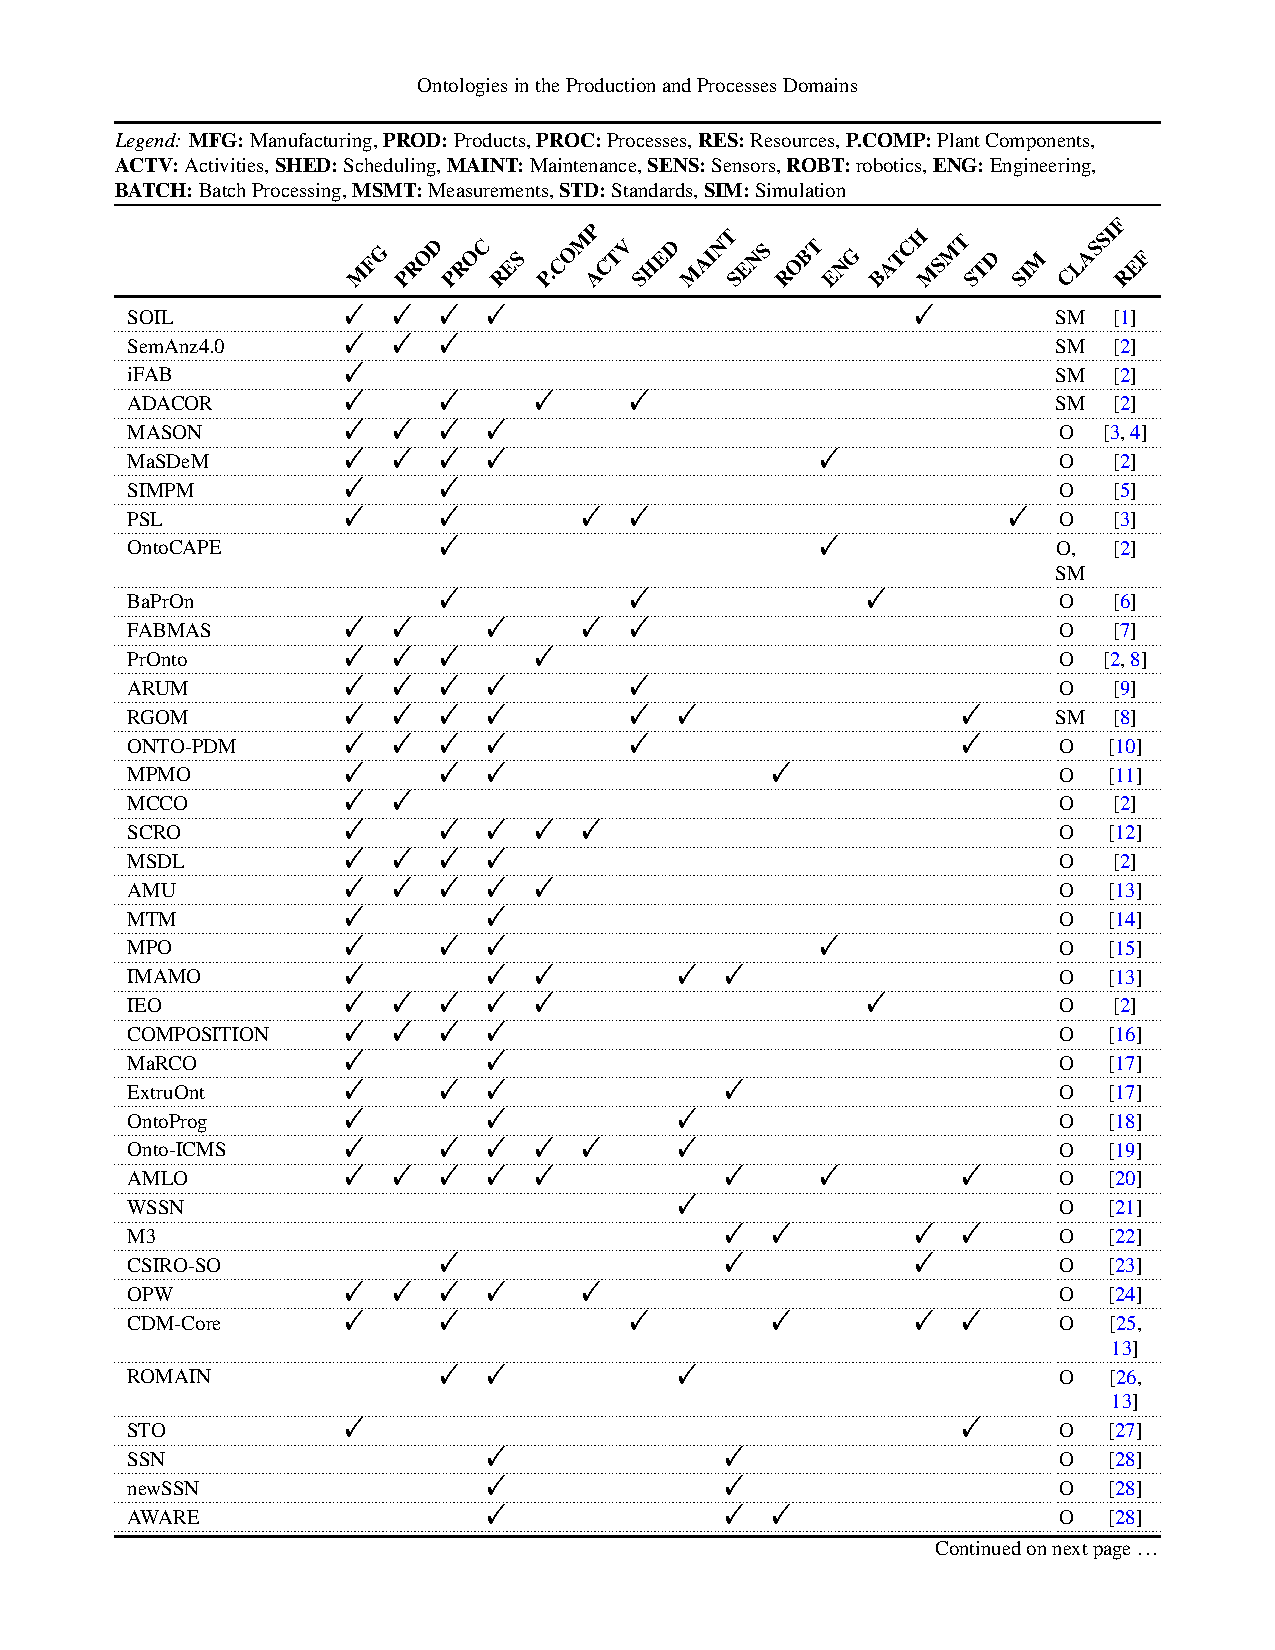
\includepdf[pages=-]{images/domainontologiestable.pdf}

\end{document}
